\chapter{Verification and Simulation}
In this chapter, we will implement the designed optimization algorithms from Chapter 5 in MATLAB and verify its correctness by checking whether the robot with optimized geometry can track the specified trim trajectories. 
The first stage hull optimization algorithm provides us a local optimum of the hull configuration. The conventional robot design specifications will be satisfied in the first design phase. Then we execute the actuator optimization codes on basis of this hull configuration and it will give us a locally optimal configuration of actuators. Two groups of actuator configuration will be exemplarily tested including 6 thrusters and 4 fins with 2 thrusters. We choose these two configurations because the number of actuators is equal to the degrees of freedom. We will visualize the robot hull and the actuator placement in MATLAB to give us an intuitive view of the unconventional actuator placement.  
The trim kinematic specifications are given in Table~\ref{table:TrimValues}. 
We expect the robot to track these specified seven trim trajectories in 200 seconds. 
\begin{table}
\centering
\caption{Trim trajectories specifications}
\begin{tabular}{| c | c | c | p{2cm} |}
\hline
Time(s)&$||\vec{v}_{\mathcal{T}}||$ (m/s)&$\dot{\psi}_{\mathcal{T}}$ (rad/s)&$\gamma_{\mathcal{T}}$ (rad)\\ \hline
0-40&2&0&0\\ \hline
40-60&2&0.0803&0 \\ \hline
60-80&2&0.0803&19.5 \\ \hline
80-120&2&0&19.5 \\ \hline
120-140&2&-0.0803&19.5 \\ \hline
140-160&2&-0.0803&0 \\ \hline
160-200&2&0&0 \\ \hline
\end{tabular}
\label{table:TrimValues}
\end{table}  

It is necessary to check whether the robot can realize the tracking goal of the specified trim trajectories (kinematic specifications) under the current geometric structure. Based on the optimal actuator configuration, we build the robot dynamics and then linearize it in terms of the the seven trim trajectories in the Table~\ref{table:TrimValues}. Then we design the switched LQR control law using the method in Chapter 4 for the seven linearized systems. The trajectory tracking will be simulated with and without actuator saturation in MATLAB/Simulink, respectively.  

Our idea to design the robot based on the trim kinematic specifications can be interpreted as training the robot structure using the trajectory datasets. Using this concept from statistics and machine learning, we perform the third group of simulation where we use one steeper trim trajectory to train the 6 thruster configuration and then test generalization with an untrained trajectory set, i.e. one for which the configuration was not optimized. 

\section{Simulation for 6 Thrusters}
For the first simulation testing, we specify that the robot only has 6 thrusters as actuators. We choose the pure thruster configuration mainly due to the following three reasons: 
\begin{itemize}
\item There exists a special discrete decision variable $b_{T}$ in the thruster decision variables group $\mathfrak{d}_{P}$. The spin direction $b_{T}$ does not take apart in the main iterative optimization loop;
\item The input mapping matrix $\emph{\textbf{B}}_{a}$ consisting merely of thrusters does not depend on the robot's dynamics states, i.e., it is not trim trajectory-determined;
\item The underwater structure with pure thrusters configuration is comparable to the multicopters discussed in~\cite{Du2016}.  
\end{itemize}

In this case, the condition number corresponding to the geometric configuration at
the last iteration (68) is the smallest. Thus, we take the geometric values from the last iteration. Figures~\ref{FIG:GeoVisualFinThrusterT11} and~\ref{FIG:GeoVisualFinThrusterT12} visualize the final result of the thruster locations from the anterior view and posterior view, respectively. The hull is drawn as a hollow cylinder with length $l_{H}$ and radius $r_{H}$ which come from the results of the hull optimization. In the hull, the body frame $\lbrace b \rbrace$ is plotted where the red arrow represents its x-axis, the green arrow represents the y-axis and the blue arrow denotes the z-axis. We use arrow line segment to represent the thrusters' geometric information. All of them are unit vectors whose starting point is attached on the hull surface representing their positions $\vec{r}_{T,1}, \cdots, \vec{r}_{T,6}$ and the arrows denote their orientations $\vec{d}_{T,1}, \cdots, \vec{d}_{T,6}$. 
\begin{figure}
\center
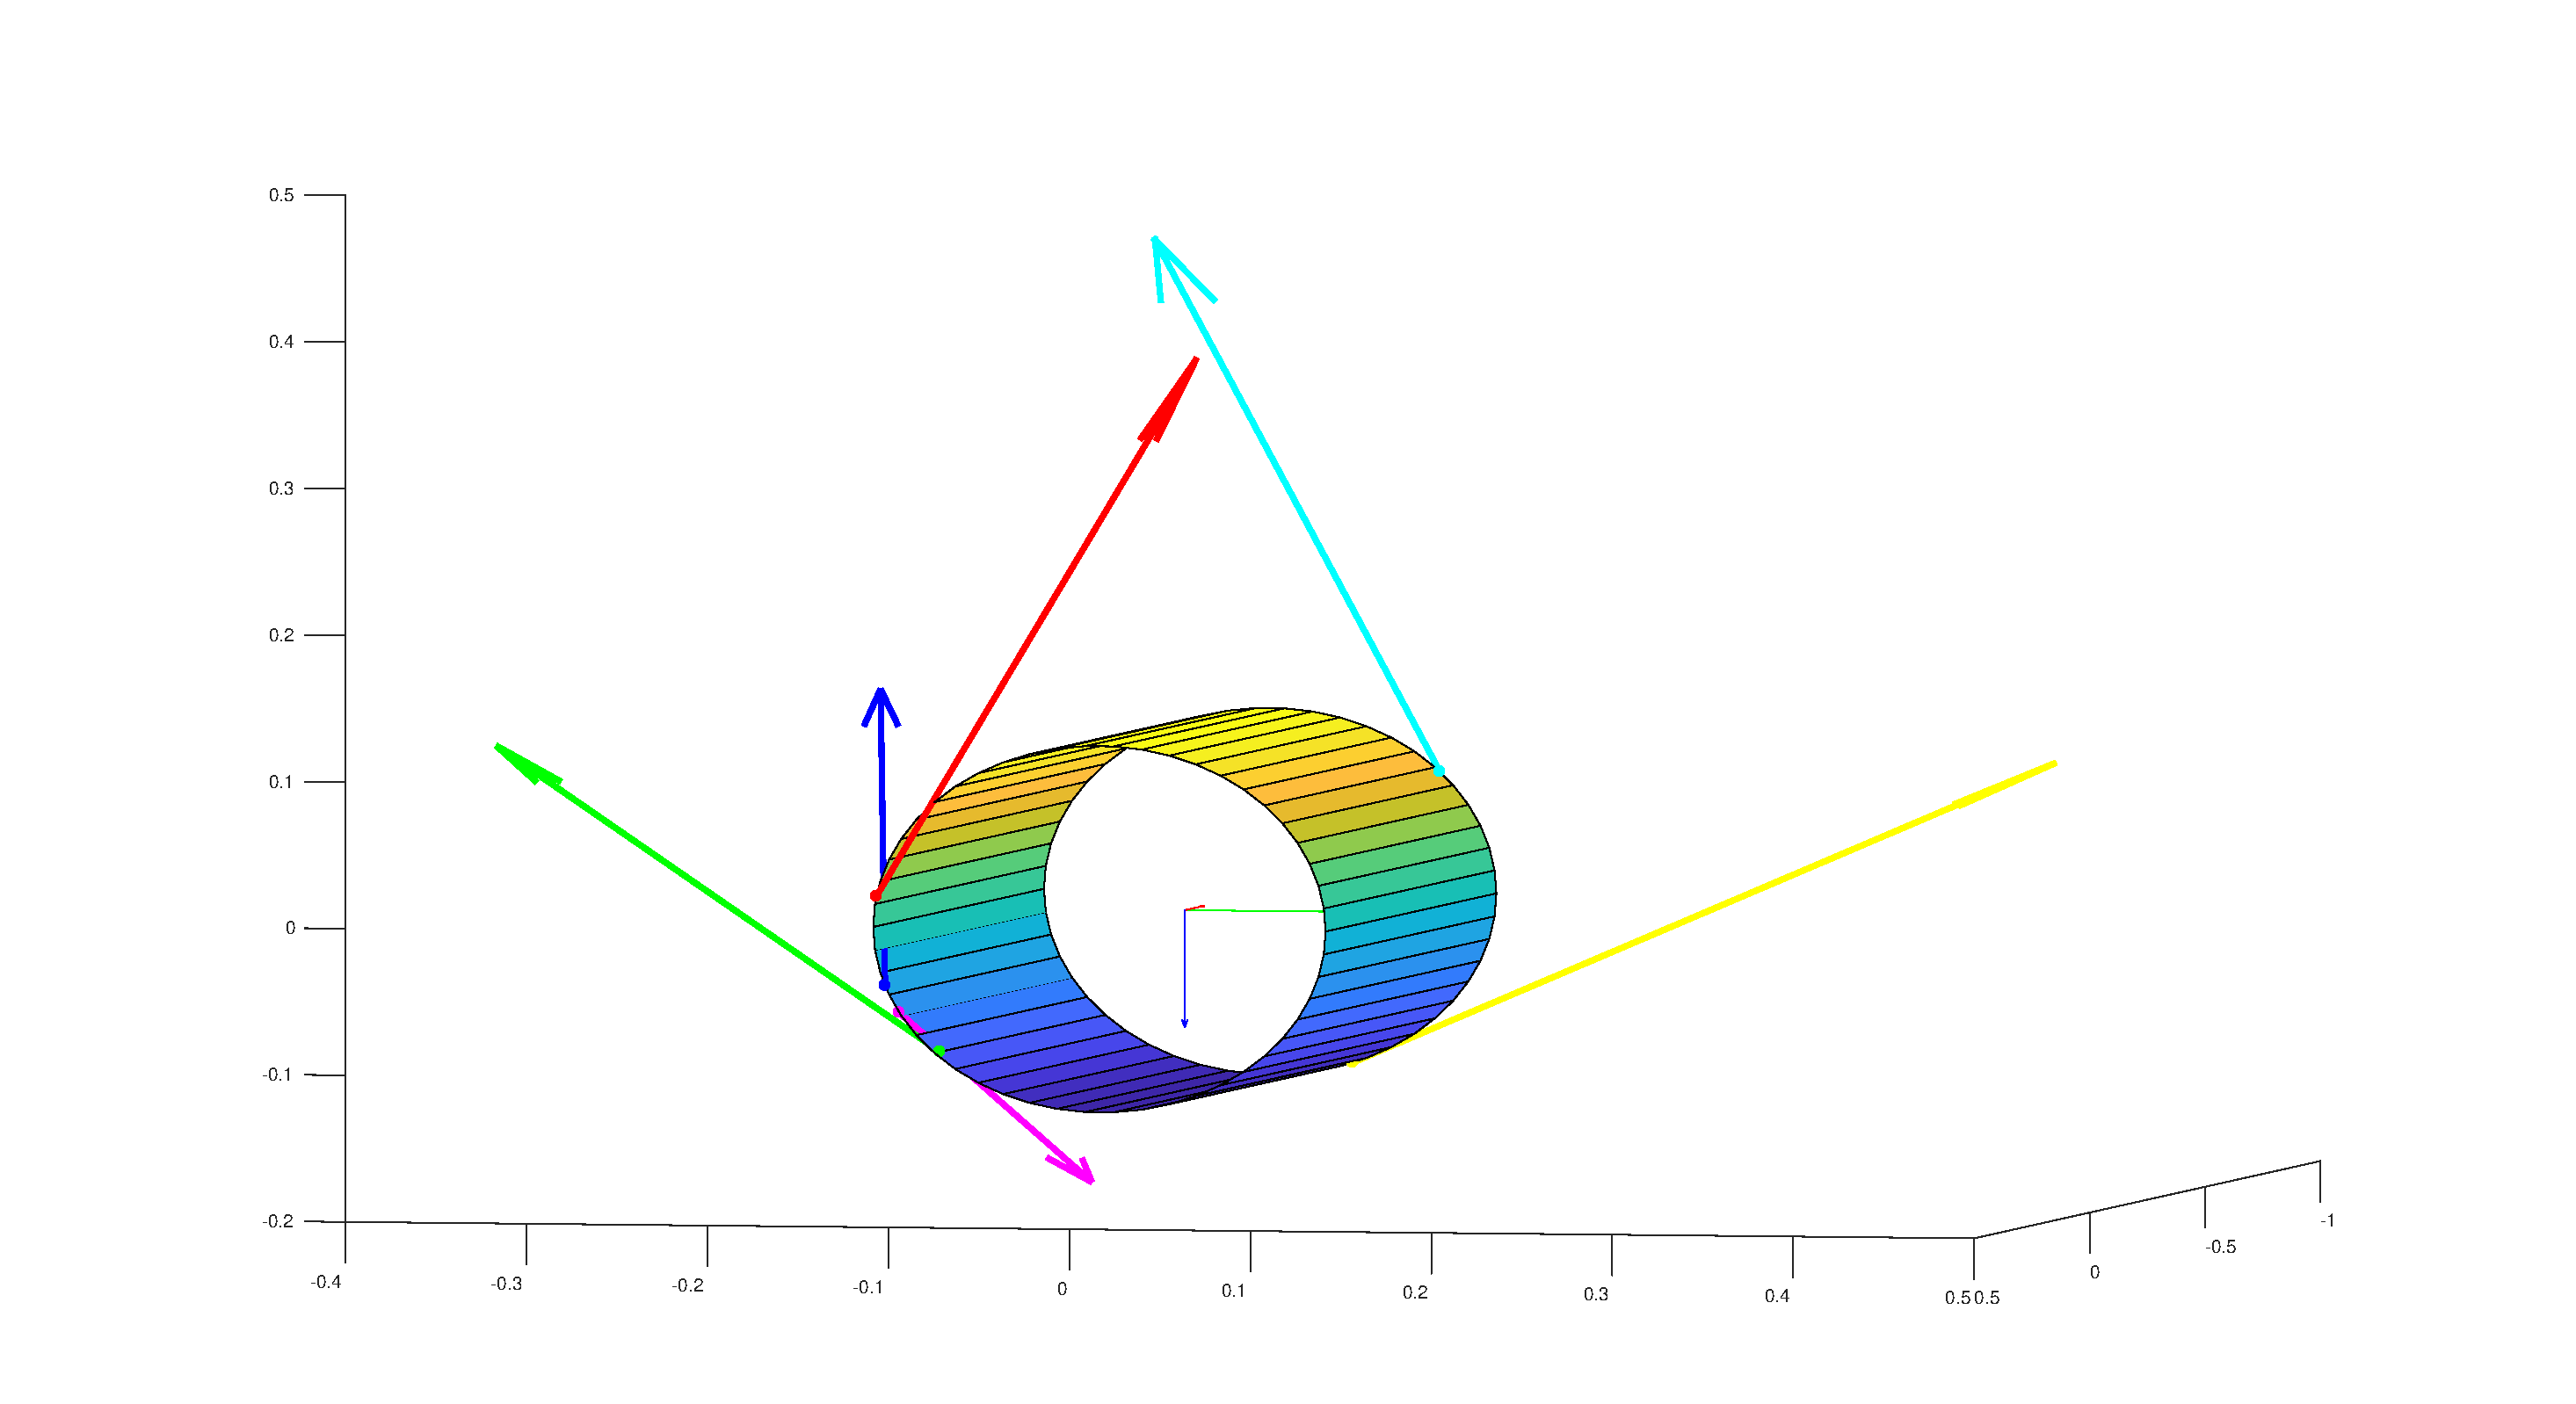
\includegraphics[width=0.9\textwidth]{GeoVisualFinThrusterT11.eps}
\caption{Visualization of optimization result (6 thrusters) perspective 1}	
\label{FIG:GeoVisualFinThrusterT11}
\end{figure}
\begin{figure}
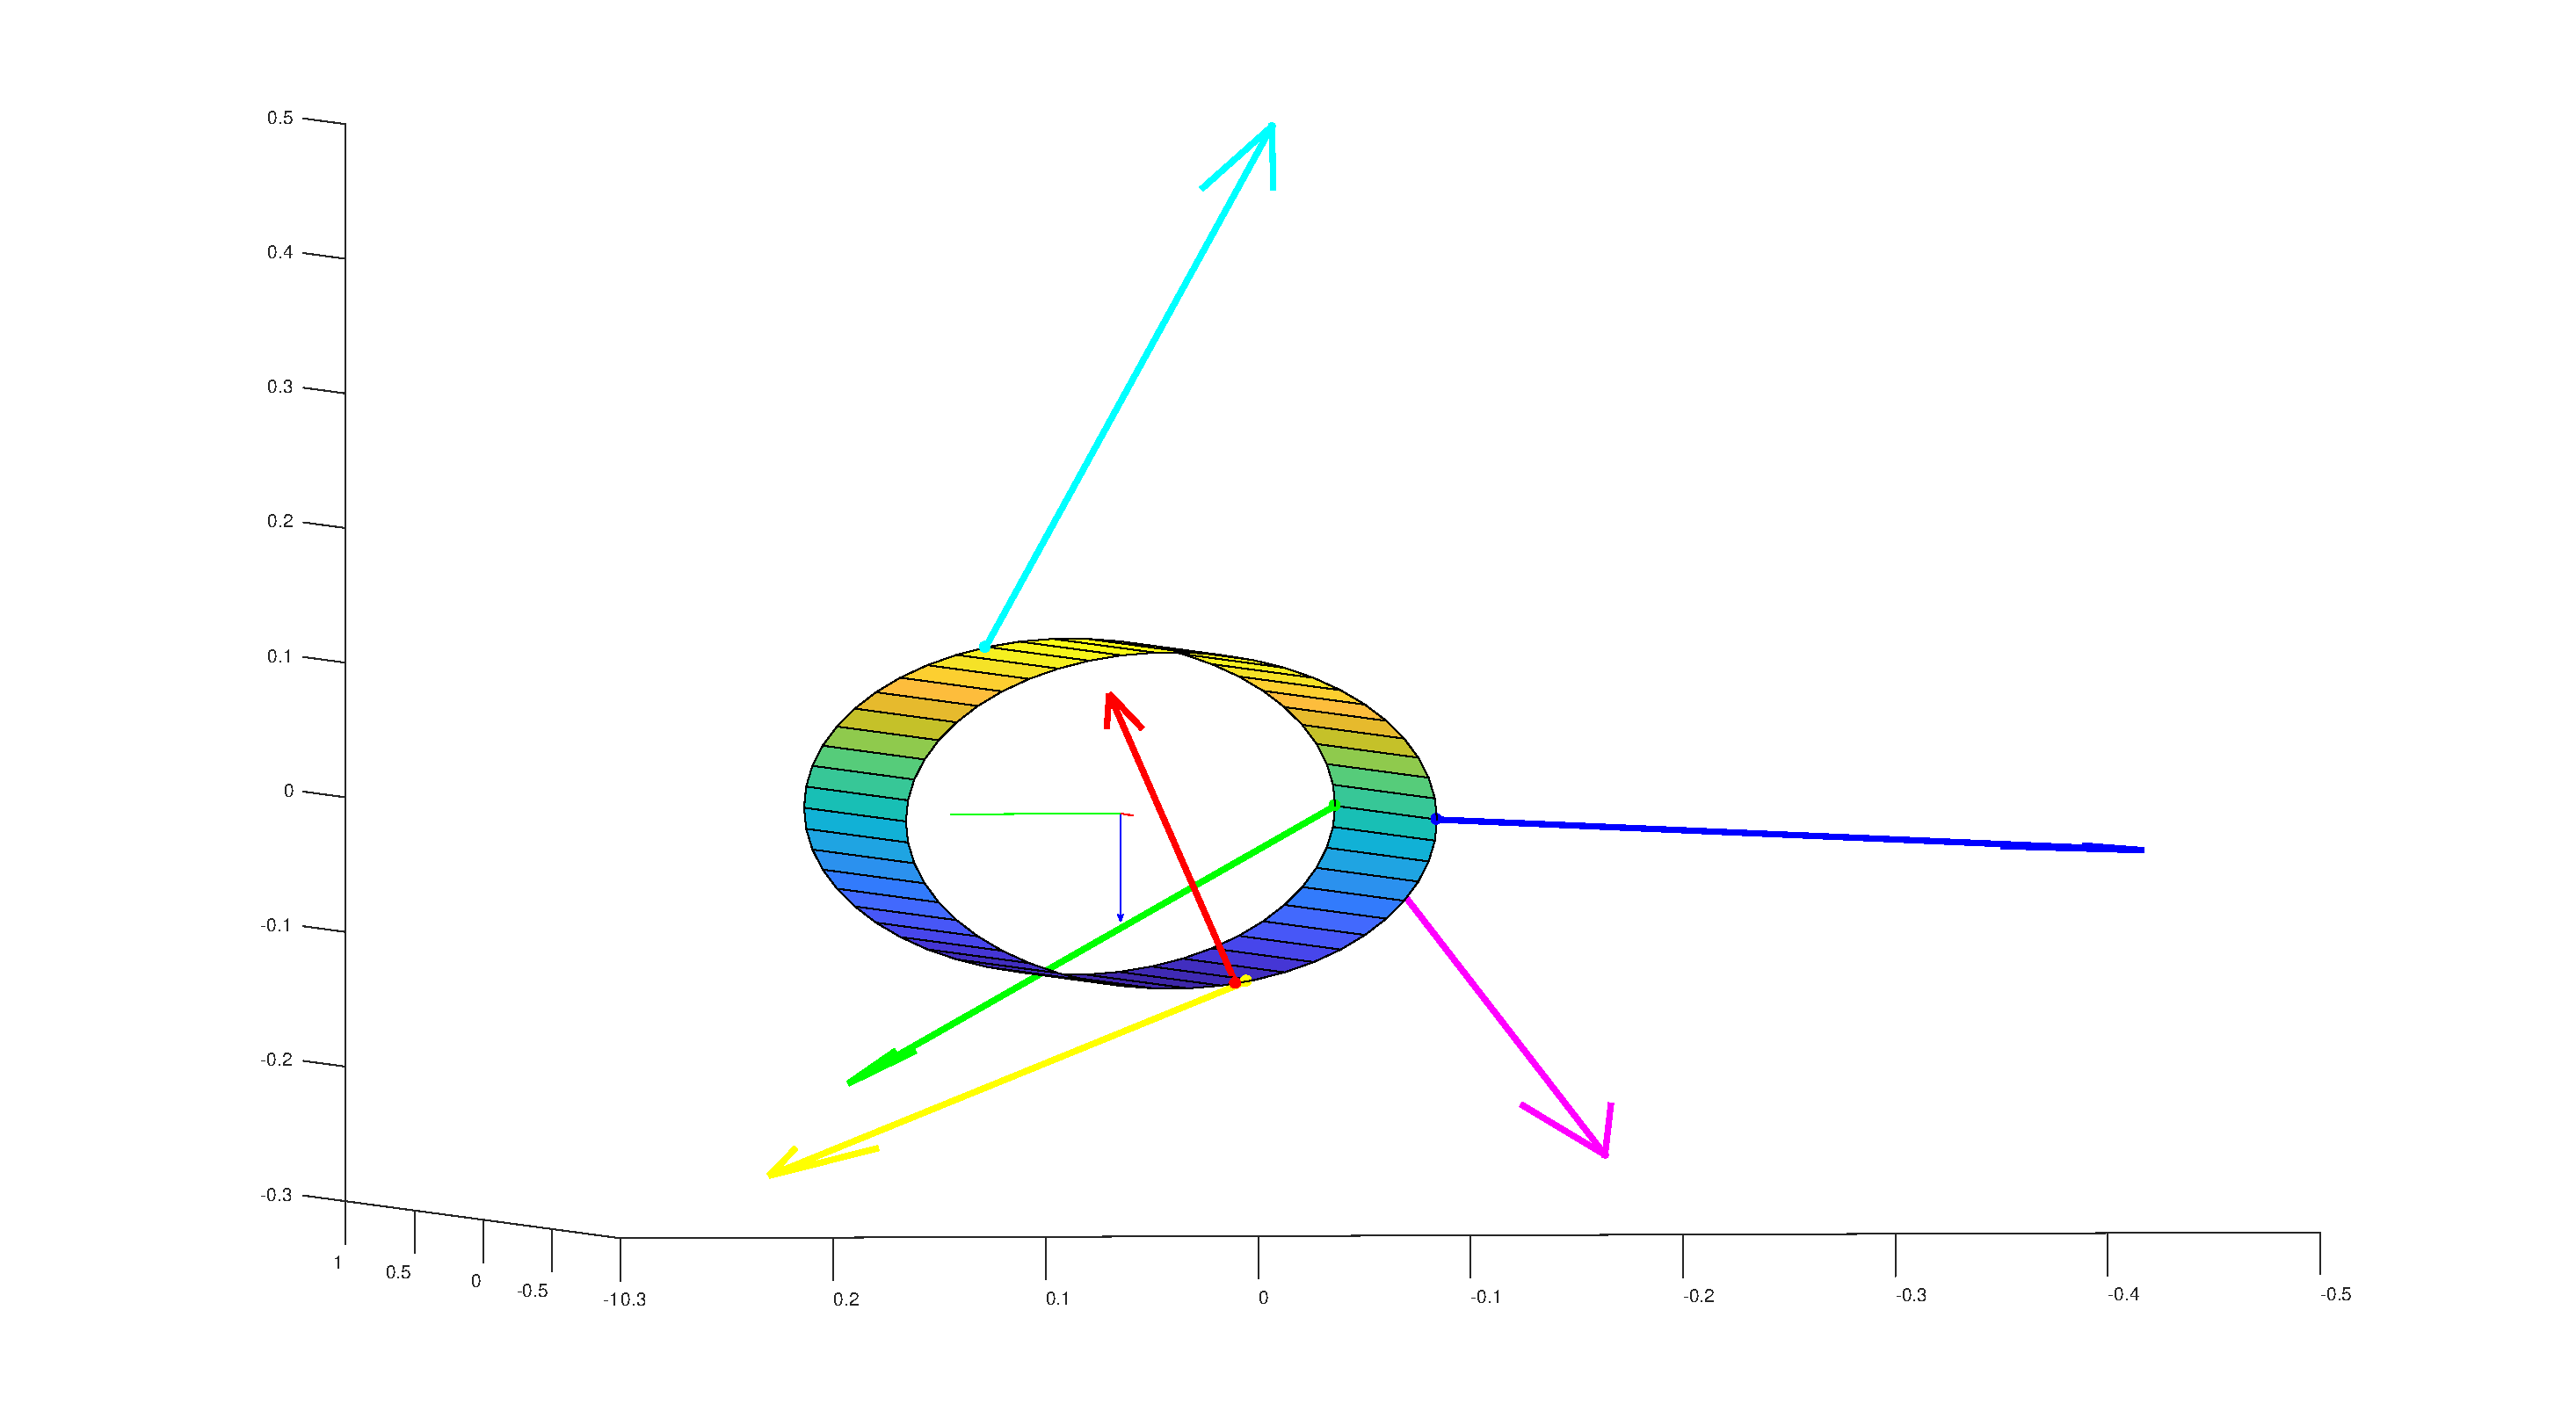
\includegraphics[width=\textwidth]{GeoVisualFinThrusterT12.eps}
\caption{Visualization of optimization result (6 thrusters) perspective 2}	
\label{FIG:GeoVisualFinThrusterT12}
\end{figure}

%%%%%%%%%%%%%%%%%%%%%%%%%%%%%%%%%%%%%%%%%%%%%%%%%%%%%%%%%%%%%%%%%%%%%%%%%%%%%%%%%
We set the value of $\epsilon$ according to the initial average norm of all trim trajectory error dynamics controllability matrices $\emph{\textbf{C}}_{E,av,init}=\dfrac{1}{7}\sum_{j=1}^{7}||\emph{\textbf{C}}_{E,j}^{1}||$, here we choose $\epsilon=0.001\emph{\textbf{C}}_{E,av,init}$. By using this $\epsilon$ value for breaking, the optimization algorithm will break only for 68 iterations, only one third of the specified maximal iterations ($k_{max}=200$). The norms of the error dynamics controllability matrices are in the order of $10^{9}$, as illustrated in Figure~\ref{FIG:ConNormT1}. They increase roughly in the first four iterations and fall down until the 18-th iteration. After that, the norm values do not change heavily and begin to converge slowly from the 50-th iteration.
\begin{figure}
\centering
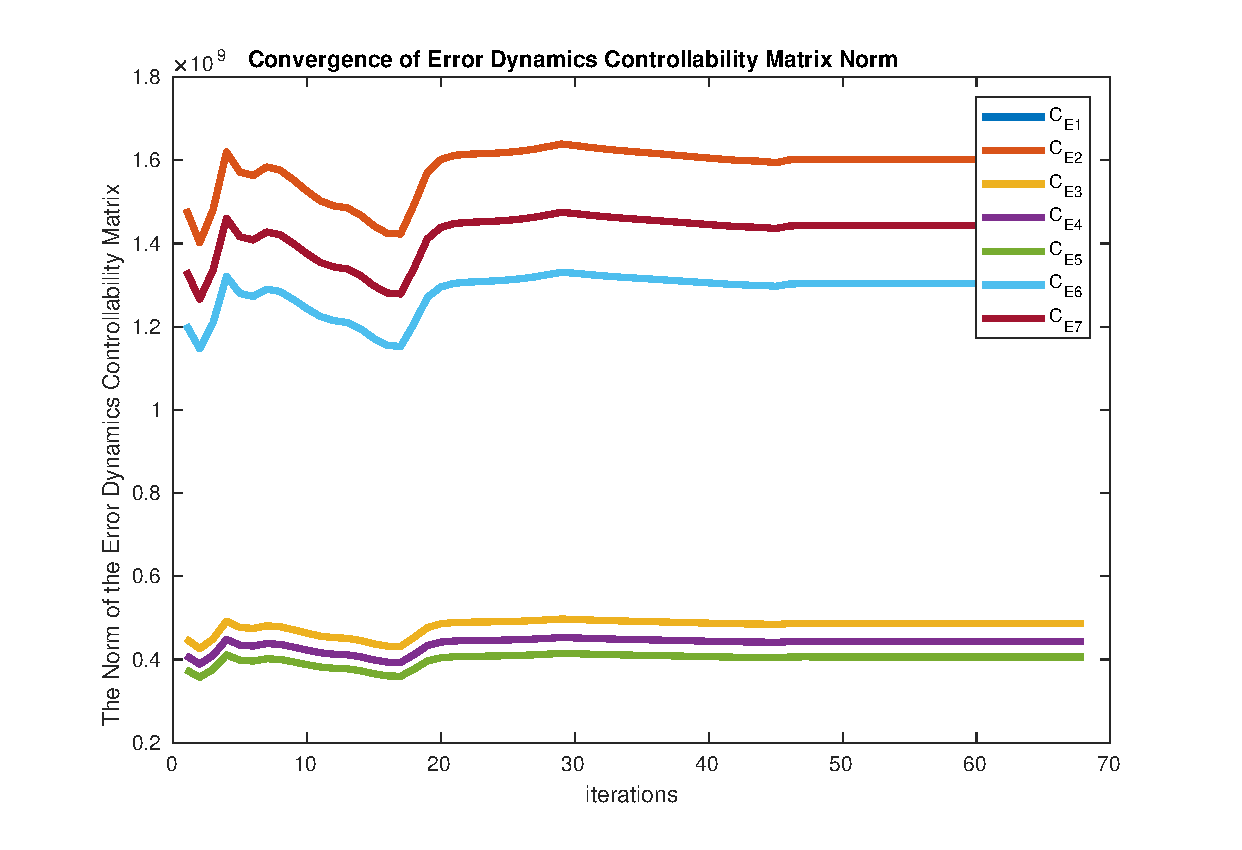
\includegraphics[width=0.75\textwidth]{ConNormT1.eps}
\caption{Convergence of error dynamics controllability matrix norm (6 thrusters)}	
\label{FIG:ConNormT1}
\end{figure}
The positions and orientations of the 6 thrusters are depicted in~\ref{FIG:ConPosInput2}. The positions and orientations of all 6 thrusters except for the thruster 2 direction vector $\vec{d}_{T,2}$ change obviously in the first 50 iterations and tend to converge from the 50-th iteration corresponding to the convergence of the controllability matrices norms. Only one direction vector's changing contributes to the norm negligibly, the optimization loop can still be broken. 

%%%%%%%%%%%%%%%%%%%%%%%%%%%%%%%%%%%%%%%%%%%%%%%%%%%%%%%%%%%%%%%%%%%%%%%%%%%%%%%%%
\begin{figure}
\centering
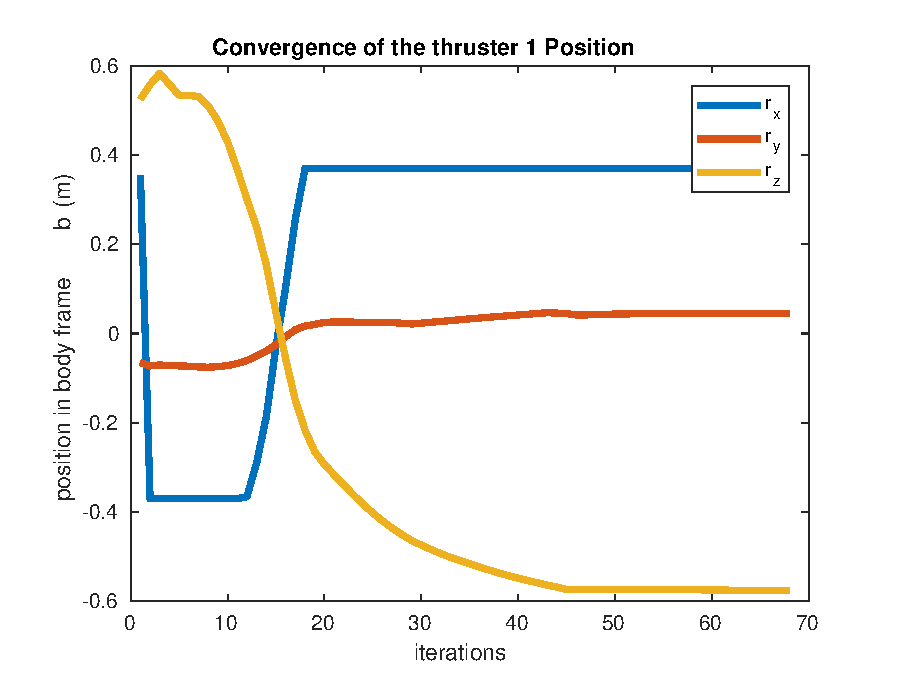
\includegraphics[width=0.45\textwidth]{ConThruster1PosT1.eps}
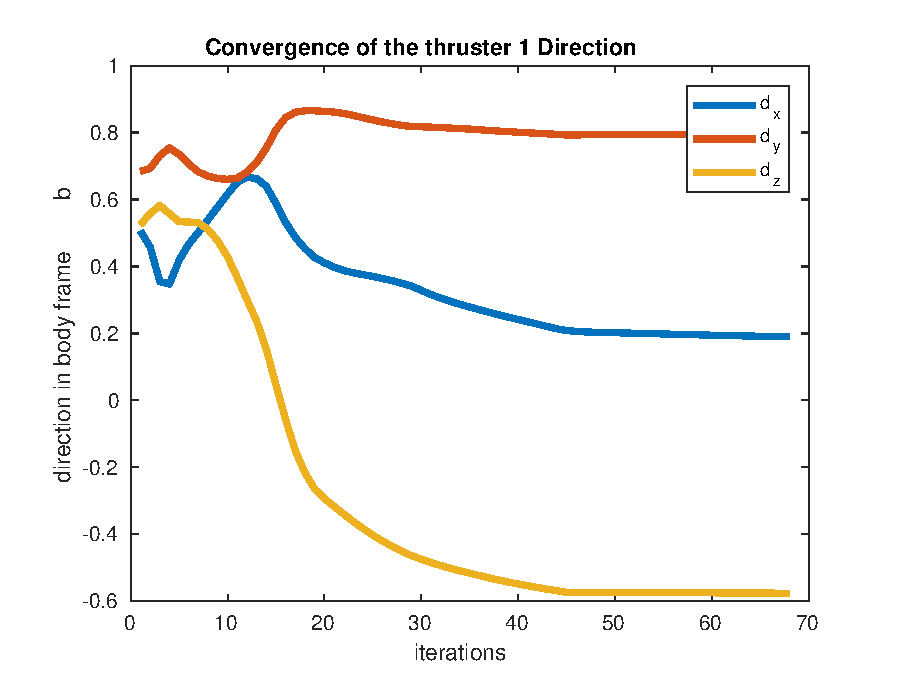
\includegraphics[width=0.45\textwidth]{ConThruster1DirT1.eps}
\caption{Convergence of position and direction of thruster 1 (6 thrusters)}	
\label{FIG:ConThrusterT11}
\end{figure}
\begin{figure}
\centering
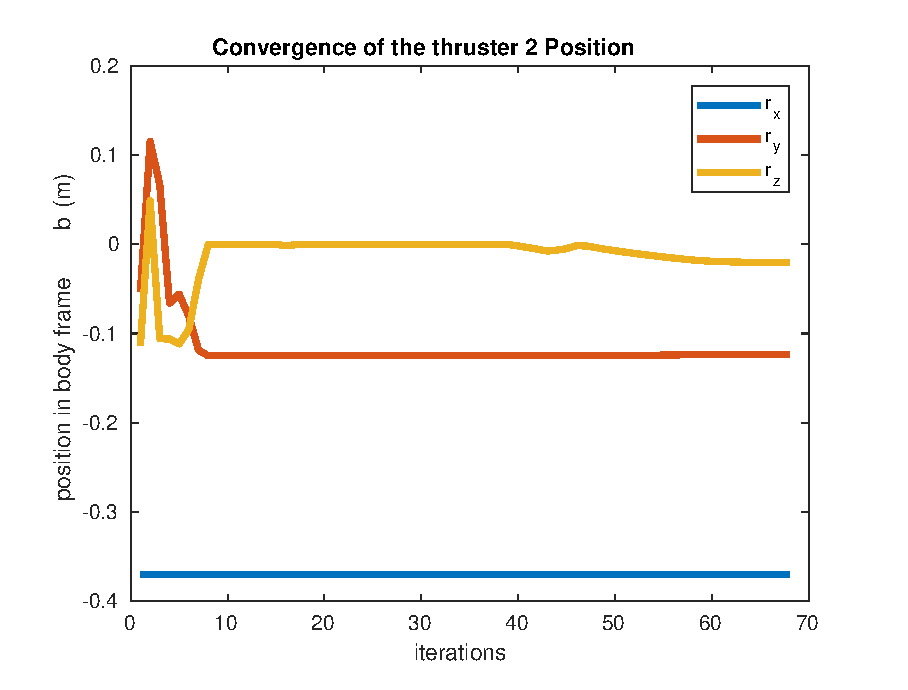
\includegraphics[width=0.45\textwidth]{ConThruster2PosT1.eps}
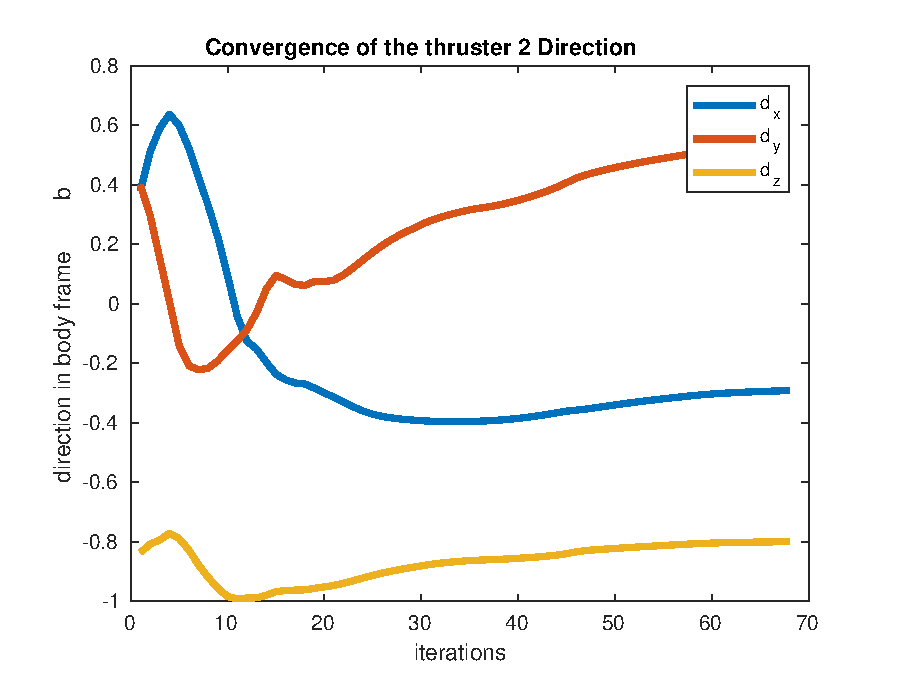
\includegraphics[width=0.45\textwidth]{ConThruster2DirT1.eps}
\caption{Convergence of position and direction of thruster 2 (6 thrusters)}	
\label{FIG:ConThrusterT21}
\end{figure}
\begin{figure}
\centering
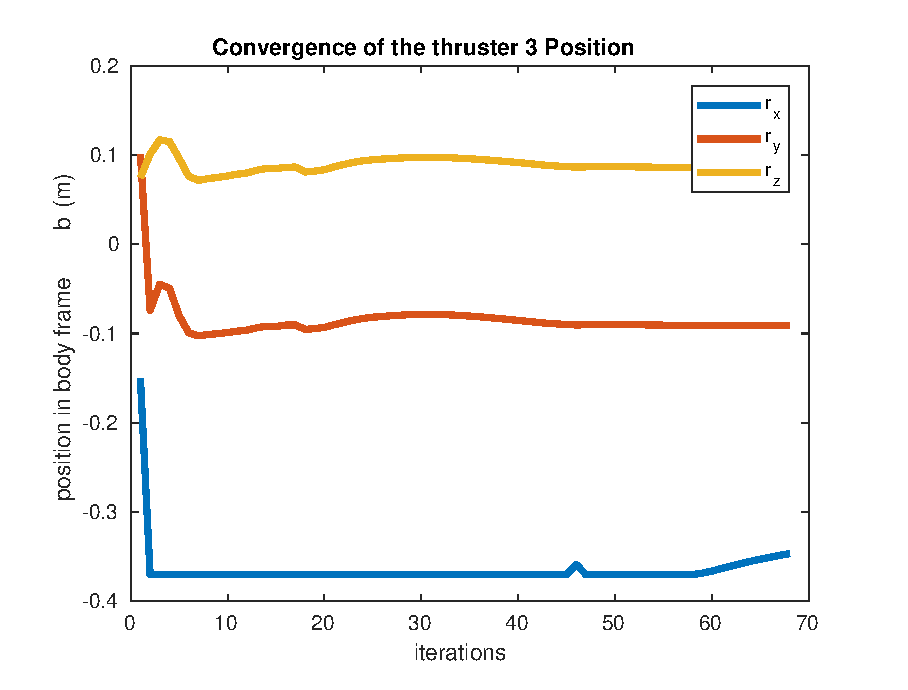
\includegraphics[width=0.45\textwidth]{ConThruster3PosT1.eps}
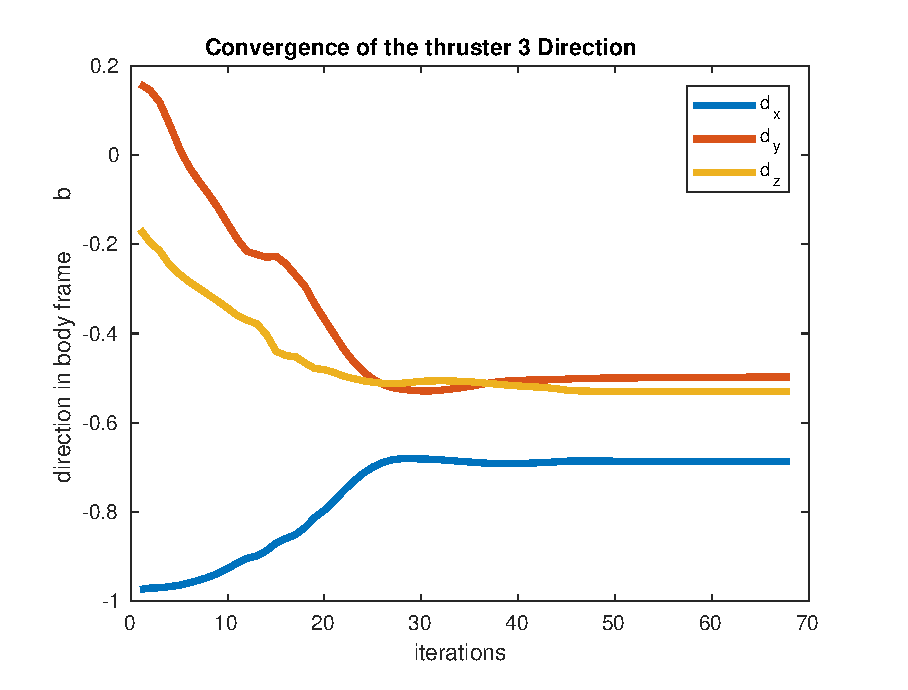
\includegraphics[width=0.45\textwidth]{ConThruster3DirT1.eps}
\caption{Convergence of position and direction of thruster 3 (6 thrusters)}	
\label{FIG:ConThrusterT31}
\end{figure}
\begin{figure}
\centering
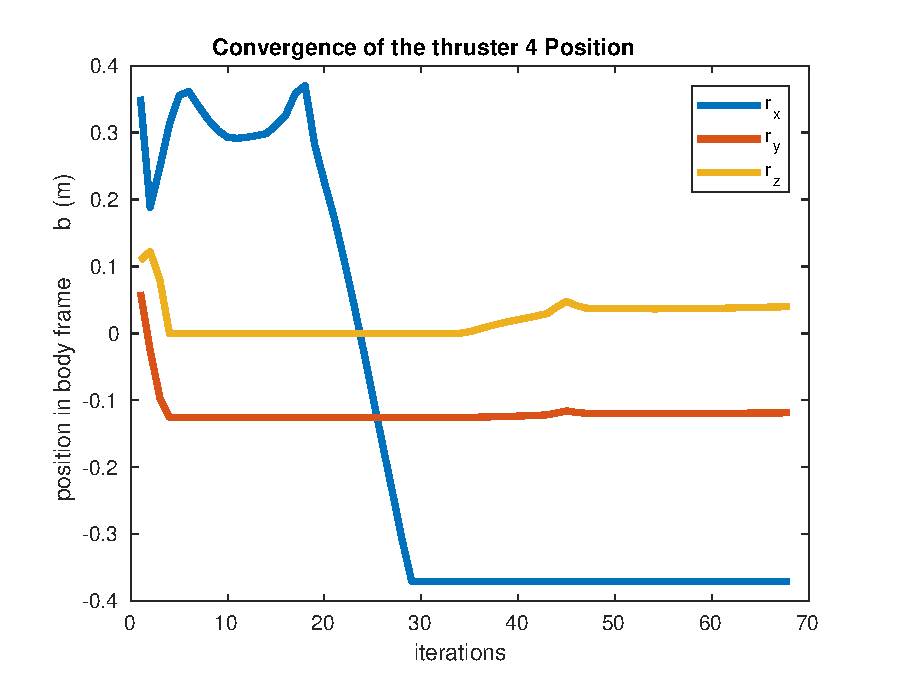
\includegraphics[width=0.45\textwidth]{ConThruster4PosT1.eps}
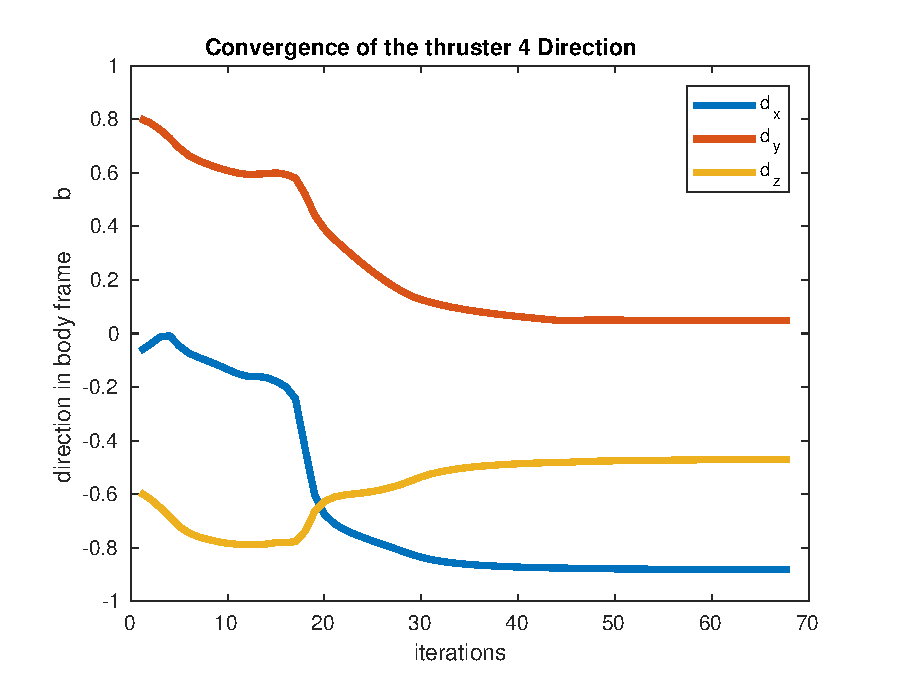
\includegraphics[width=0.45\textwidth]{ConThruster4DirT1.eps}
\caption{Convergence of position and direction of thruster 4 (6 thrusters)}	
\label{FIG:ConThrusterT41}
\end{figure}
\begin{figure}
\centering
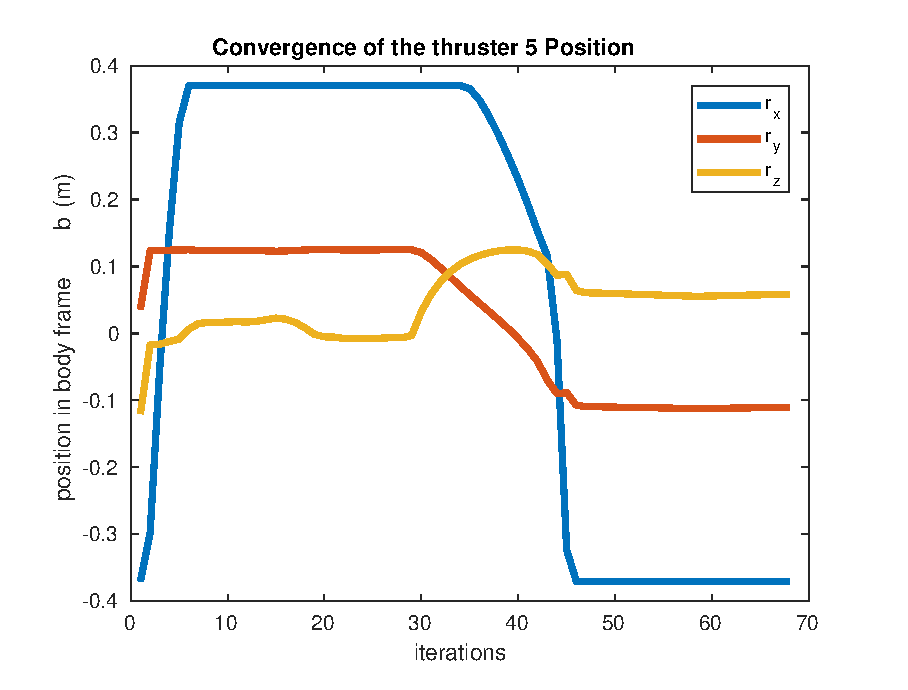
\includegraphics[width=0.45\textwidth]{ConThruster5PosT1.eps}
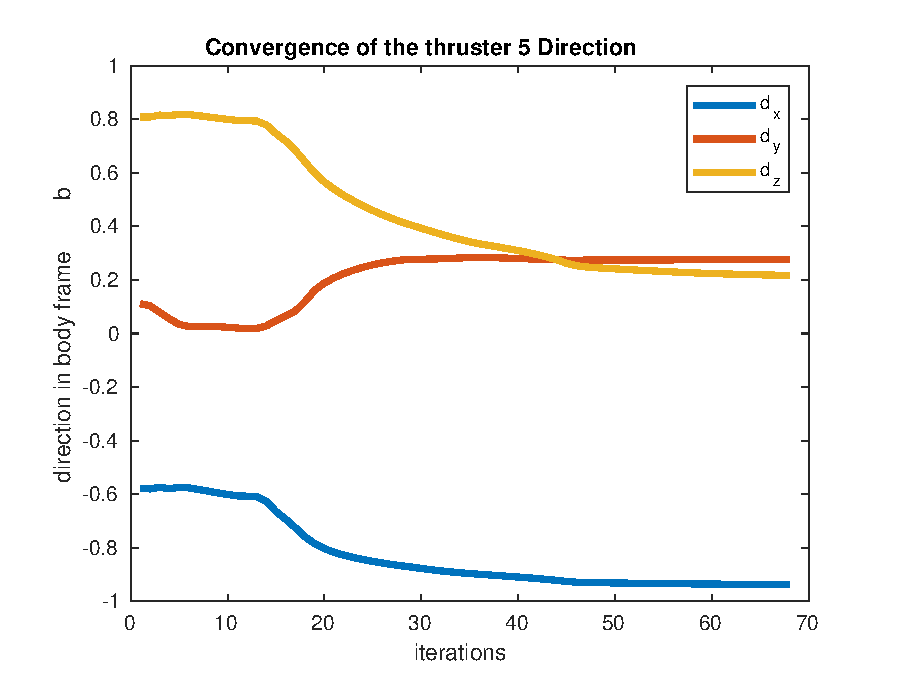
\includegraphics[width=0.45\textwidth]{ConThruster5DirT1.eps}
\caption{Convergence of position and direction of thruster 5 (6 thrusters)}	
\label{FIG:ConThrusterT51}
\end{figure}
\begin{figure}
\centering
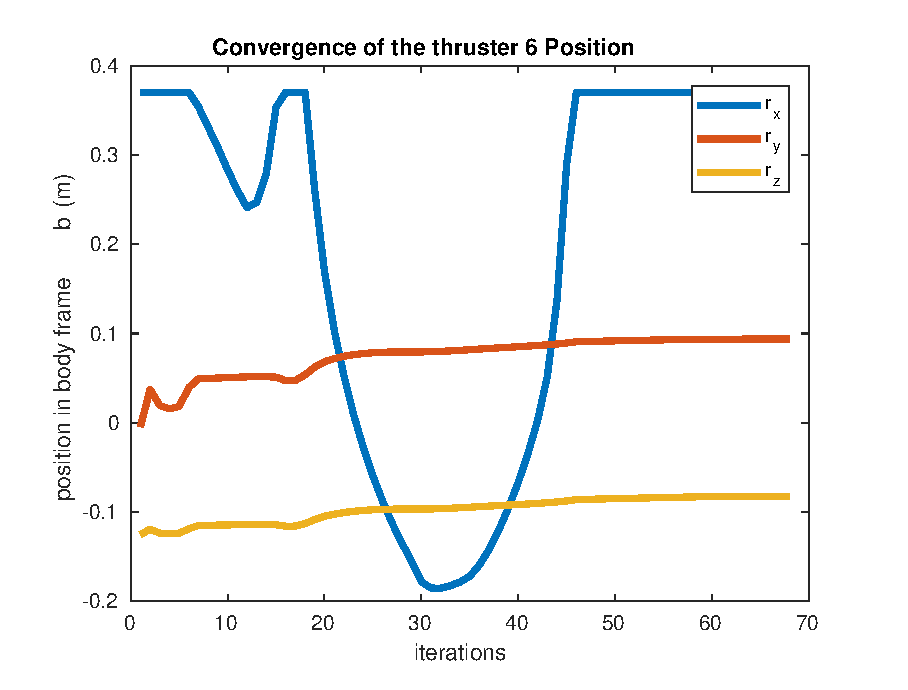
\includegraphics[width=0.45\textwidth]{ConThruster6PosT1.eps}
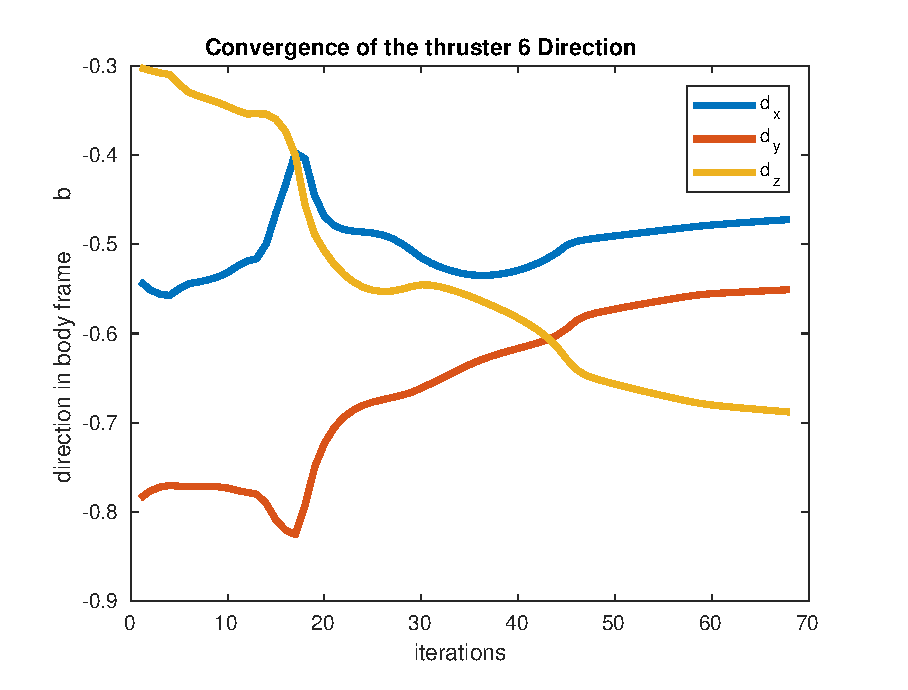
\includegraphics[width=0.45\textwidth]{ConThruster6DirT1.eps}
\caption{Convergence of position and direction of thruster 6 (6 thrusters)}	
\label{FIG:ConThrusterT61}
\end{figure}

Recall that we have three optimization steps: control input optimization, position optimization and orientation optimization. As depicted in Figure~\ref{FIG:ConInputPosT1}, the control input objective function (~\ref{EQ:OPTInput}) value $fval_{input}$ increases from 210 to 380 and then decreases significantly to 50 at the iteration 30. After that, it falls down slightly until the last iteration. The convergence value of $fval_{input}$ is merely one fifths of the initial objective value, namely 40. The position optimization objective value $fval_{pos}$ starts also approximately from 110 and decreases to 10 in 68 optimization loops.

\begin{figure}
\center
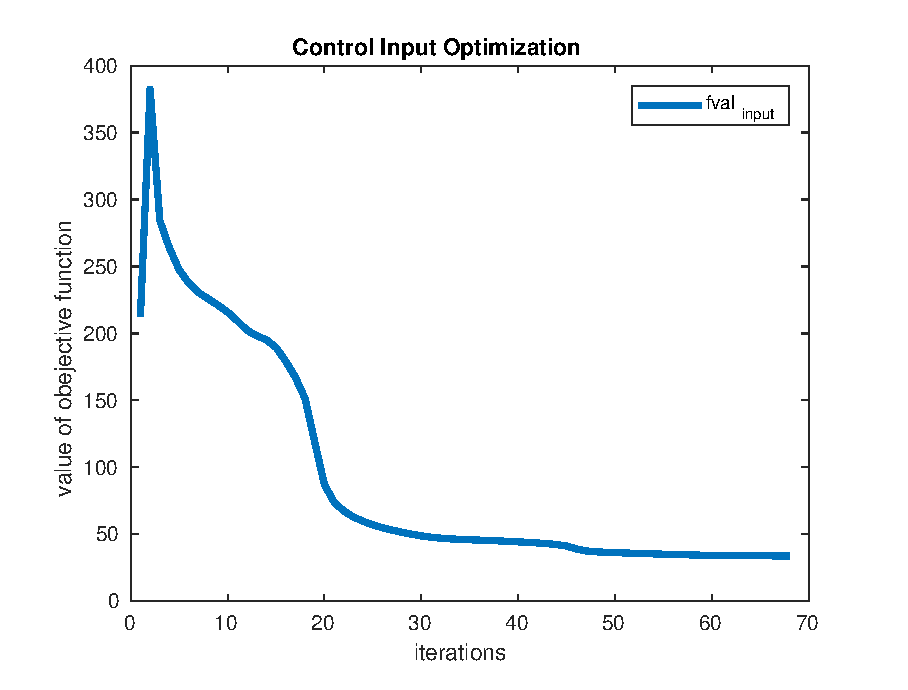
\includegraphics[width=0.49\textwidth]{ConInputT1.eps}
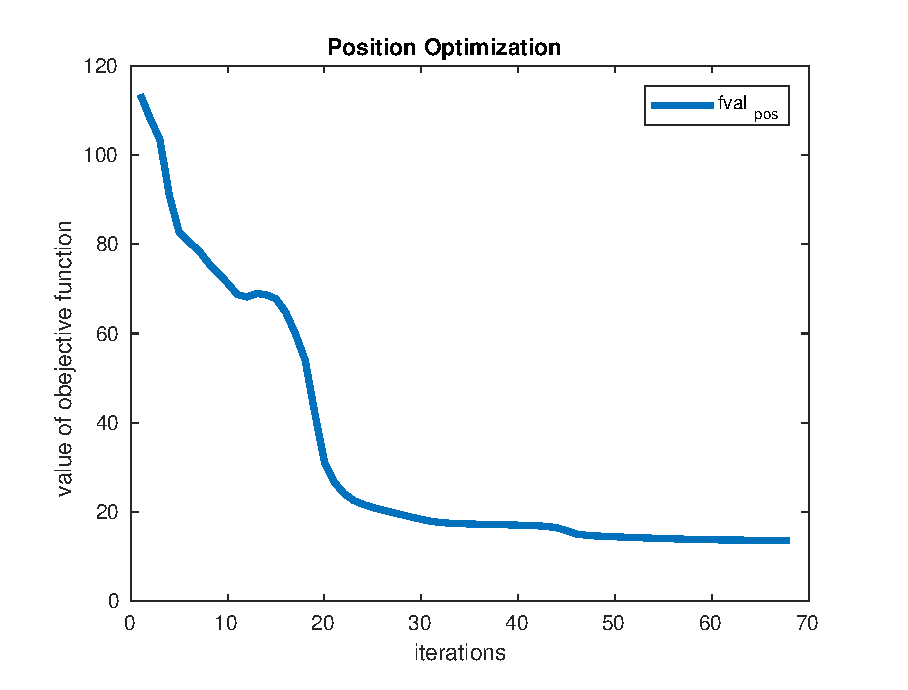
\includegraphics[width=0.49\textwidth]{ConPosT1.eps}
\caption{Value of objective functions (6 thrusters)}	
\label{FIG:ConInputPosT1}
\end{figure}
\newpage
We build the switched LQR controller using the state cost and input cost matrices from Table~\ref{table:QParameters} and~\ref{table:RParameters for 6 thrusters}. 
Under the current configuration, we want the robot to track the specified 7 trim trajectories in~\ref{table:TrimValues}. As illustrated in~\ref{FIG:TrackUnsatT1}, the robot can realize perfect tracking without actuator constraint. When we add the actuator saturation, as depicted in Figure~\ref{FIG:TrackSatT1}, the robot is able to keep the trim paths roughly.
  
\begin{table}
\centering
\small
\caption{State cost matrices }
\begin{tabular}{| c | c | c | p{0.5cm} |}
\hline
Index&$\mathcal{Q}_{E}$\\ \hline
1&diag([1000,1000,1000,300,300,300,1,1,1,1,1,1]) \\ \hline
2&diag([1000,1000,1000,300,300,300,1,1,1,1,1,1]) \\ \hline
3&diag([1000,1000,1000,300,300,300,1,1,1,1,1,1])\\ \hline
4&diag([1000,1000,1000,1,1,1,1,1,1,1,1,1]) \\ \hline
5&diag([1000,1000,1000,300,300,300,1,1,1,1,1,1])\\ \hline
6&diag([1000,1000,1000,300,300,300,1,1,1,1,1,1])\\ \hline
7&diag([1000,1000,1000,300,300,300,1,1,1,1,1,1]) \\ \hline
\end{tabular}
\label{table:QParameters}
\end{table} 
\begin{table}
\centering
\small
\caption{Input cost matrices for 6 thrusters}
\begin{tabular}{| c | c | c | c | p{0.5cm} |}
\hline
Index&$\mathcal{R}_{E}$ \\ \hline
1&diag([0.001,0.001,0.001,0.001,0.001,0.001])\\ \hline
2&diag[0.001,0.001,0.001,0.001,0.001,0.001] \\ \hline
3&diag([0.0001,0.0001,0.0001,0.0001,0.0001,0.0001])\\ \hline
4&diag([0.0001,0.0001,0.0001,0.0001,0.0001,0.0001]) \\ \hline
5&diag([0.0001,0.0001,0.0001,0.0001,0.0001,0.0001])\\ \hline
6&diag([0.0001,0.0001,0.0001,0.0001,0.0001,0.0001])\\ \hline
7&diag([0.001,0.001,0.001,0.001,0.001,0.001]) \\ \hline
\end{tabular}
\label{table:RParameters for 6 thrusters}
\end{table} 

\begin{figure}
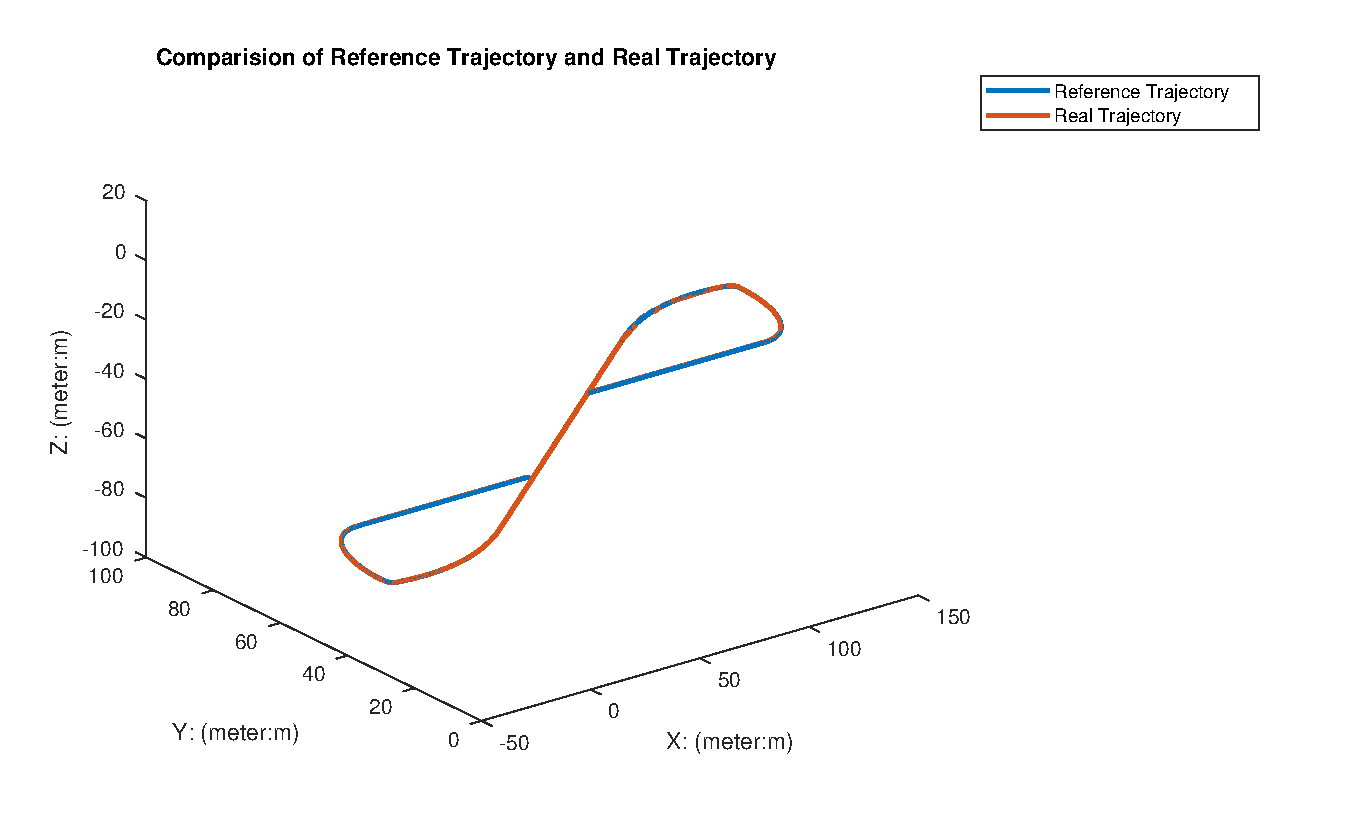
\includegraphics[width=\textwidth]{TrackUnsatT1.eps}
\caption{Comparison of desired trajectory and real trajectory (6 thrusters, no actuator saturation)}	
\label{FIG:TrackUnsatT1}
\end{figure}
\begin{figure}
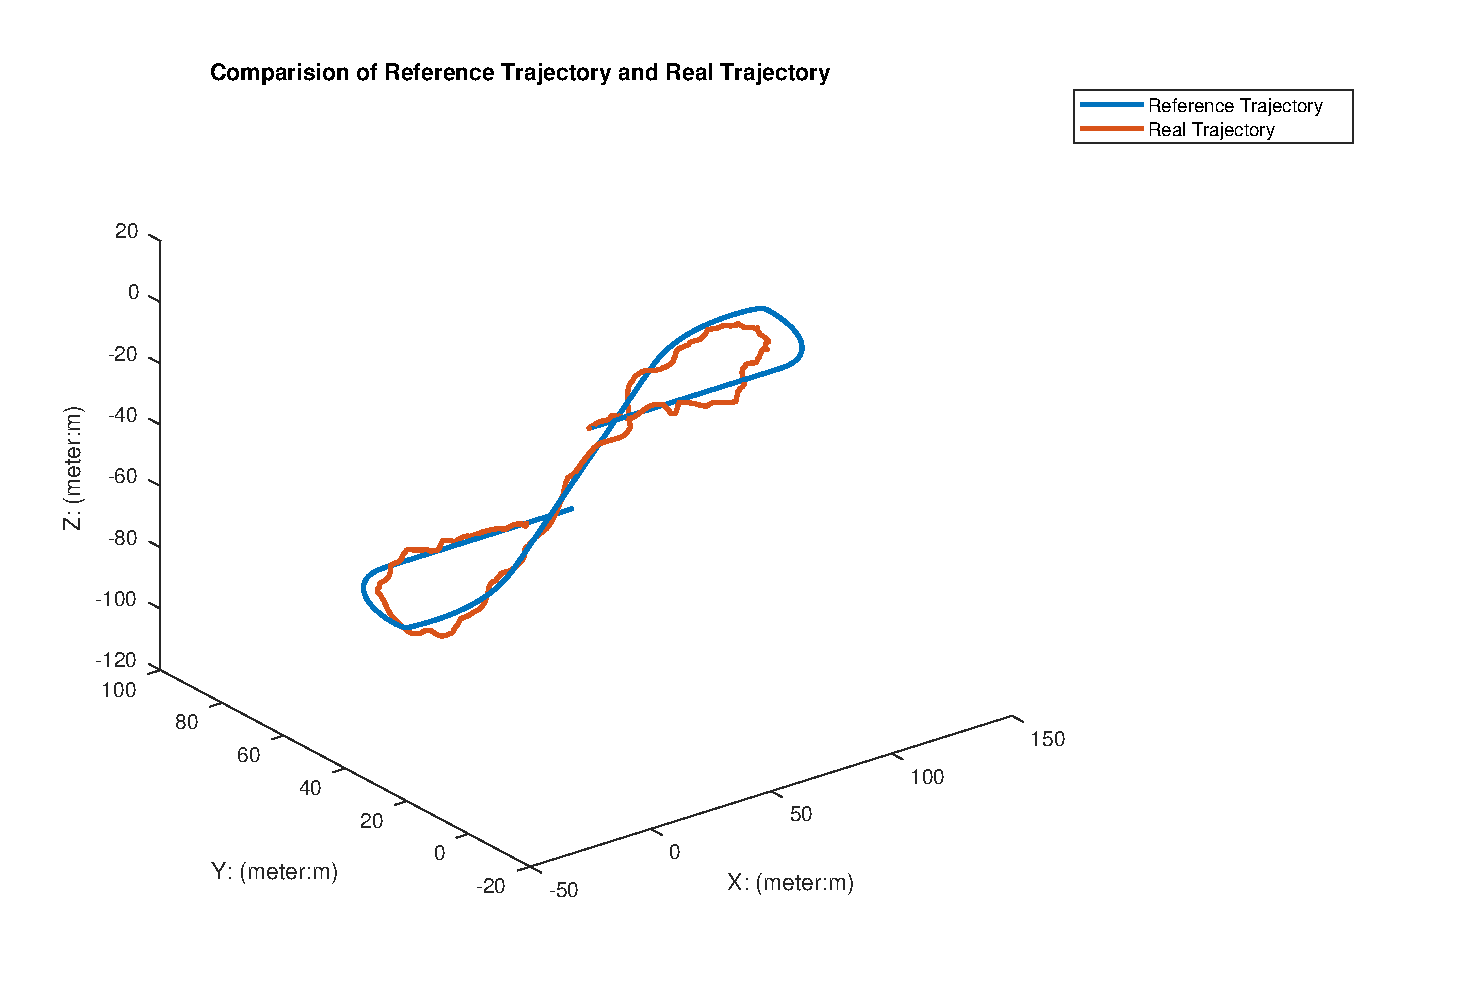
\includegraphics[width=\textwidth]{TrackSatT1.eps}
\caption{Comparison of desired trajectory and real trajectory (6 thrusters, with actuator saturation)}	
\label{FIG:TrackSatT1}
\end{figure}

\section{Training and Test for Thrusters}
As mentioned before, in this session,  we use a trim trajectory segment as training data for the optimal geometric parameters for the 6 thrusters and another trim trajectory segment for validating. The trim specifications are listed in Table~\ref{table:TrimValuesTrainTest}. The train trim trajectory possess a double trim speed ($||\vec{v}_{\mathcal{T}}||=2$ m/s) than the test trim segment ($||\vec{v}_{\mathcal{T}}||=1$ m/s). The yaw rate direction of the train trim is opposed to that of the test trajectory with nearly triple magnitude. The motion path angle $\gamma_{\mathcal{T}}$ of the train trim segment is a little smaller than that of the validation trim segment.

\begin{table}[h]
\centering
\caption{Trim Trajectory Specifications}
\begin{tabular}{| c | c | c | c | p{2cm} |}
\hline
Trim Trajectory Property&Time(s)&$||\vec{v}_{\mathcal{T}}||$ (m/s)&$\dot{\psi}_{\mathcal{T}}$ (rad/s)&$\gamma_{\mathcal{T}}$ (rad)\\ \hline
Train Trajectory&0-100&2&0.1&0.5\\ \hline
Test Trajectory&100-125&1&-0.35&0.6 \\ \hline
\end{tabular}
\label{table:TrimValuesTrainTest}
\end{table} 

General speaking, the train trim trajectory segment is more difficult to be tracked by the robot than the validation trim trajectory segment.     
 
\begin{figure}[h]
\center
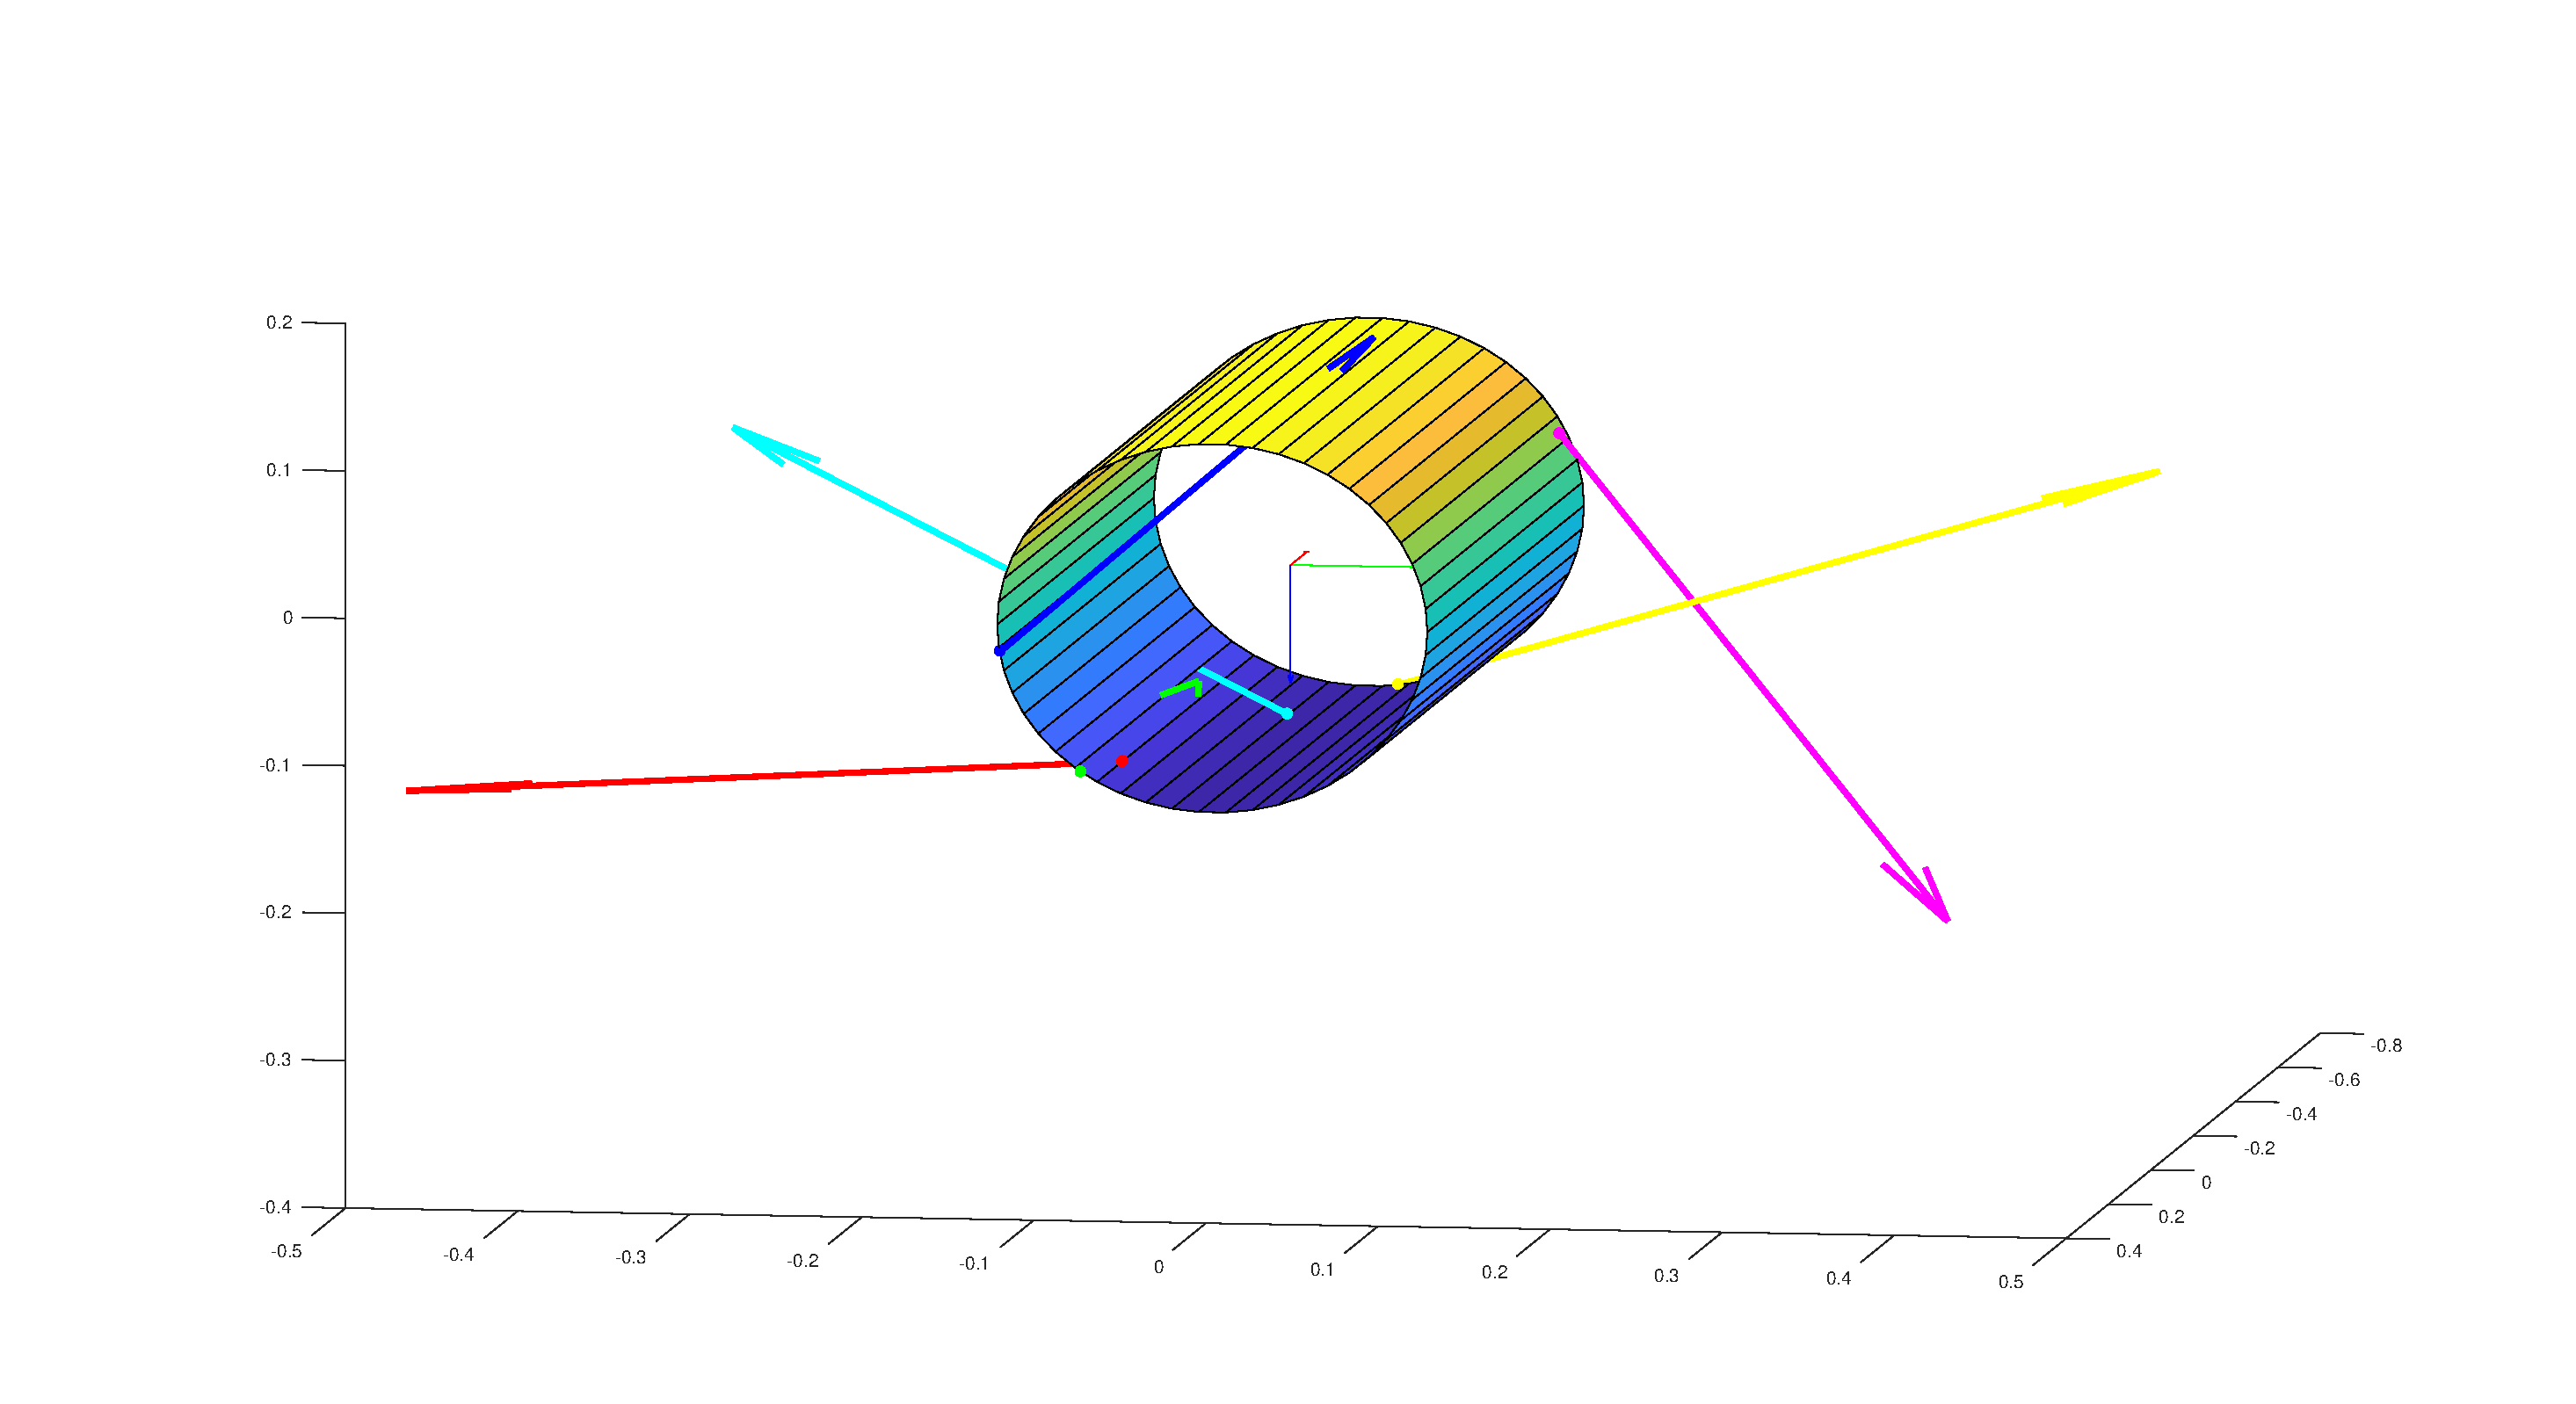
\includegraphics[width=0.9\textwidth]{GeoVisualFinThrusterTT1.eps}
\caption{Visualization of optimization result (6 thrusters, train and test) perspective 1}	
\label{FIG:GeoVisualFinThrusterTT1}
\end{figure}
\begin{figure}[h]
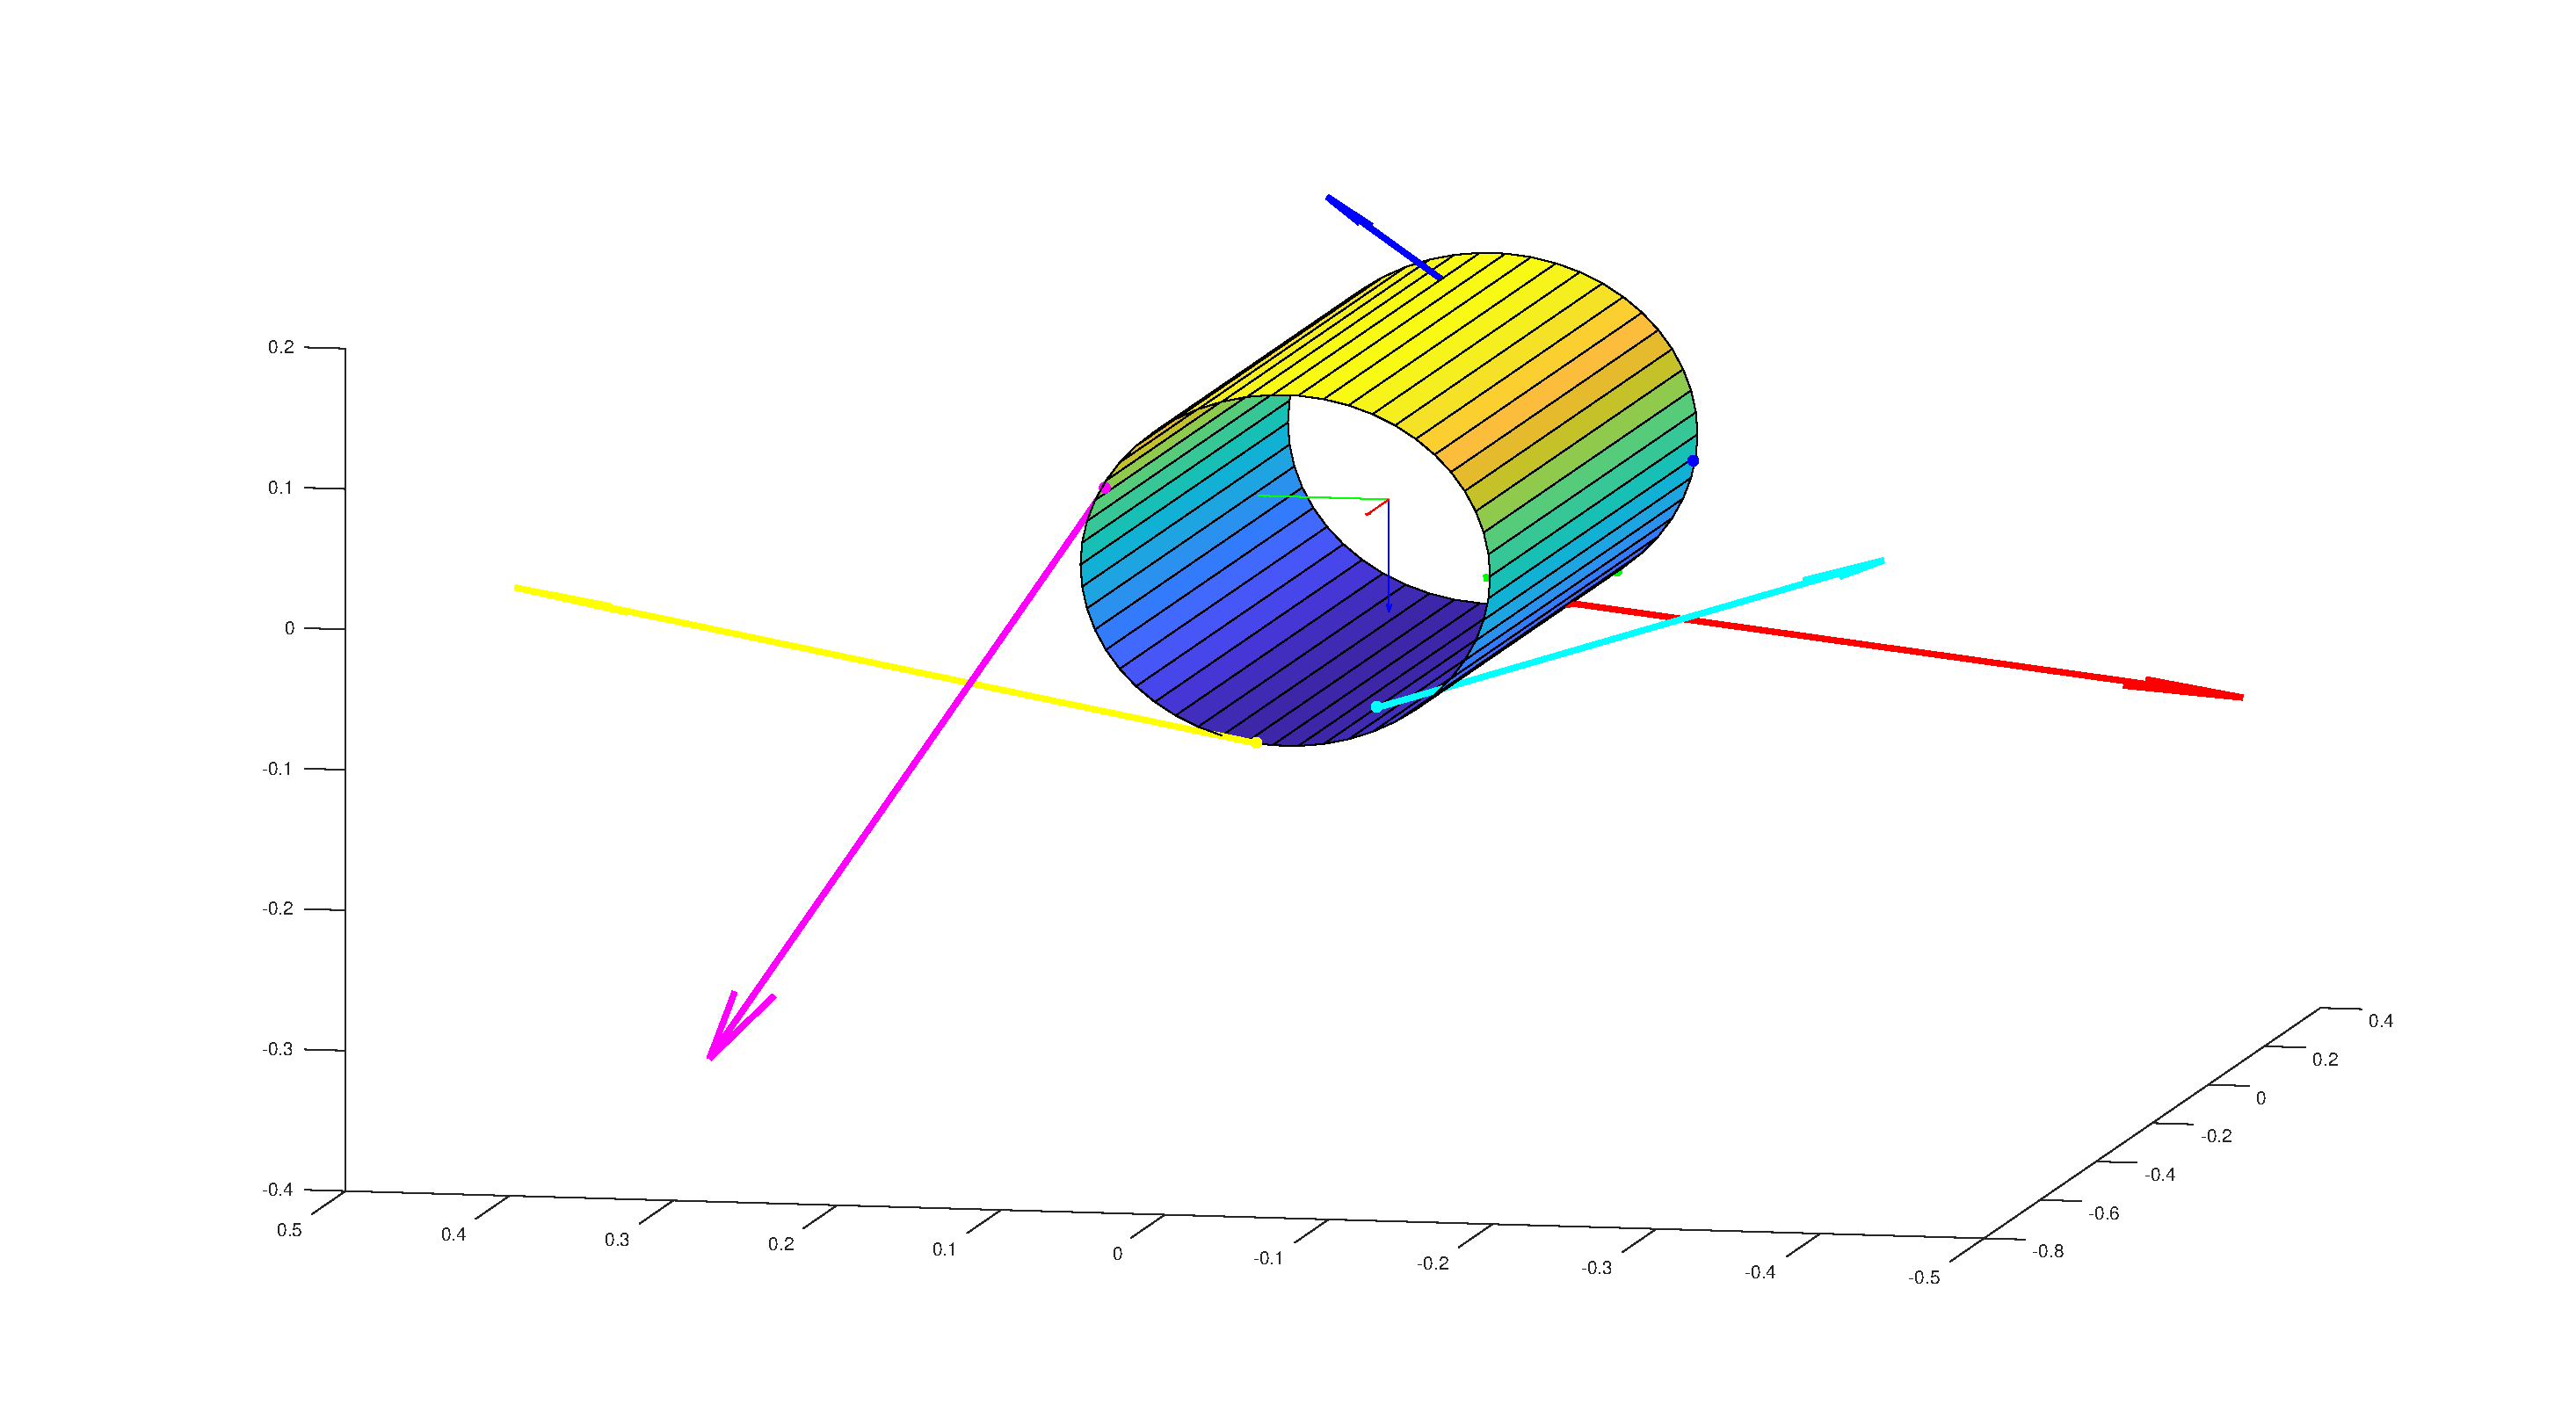
\includegraphics[width=\textwidth]{GeoVisualFinThrusterTT2.eps}
\caption{Visualization of optimization result (6 thrusters, train and test) perspective 2}	
\label{FIG:GeoVisualFinThrusterTT2}
\end{figure}
\newpage  
Since only one trim trajectory segment need to be tracked, the calculation amount is much less than the case of seven trim trajectories in the previous section. From Figures~\ref{FIG:ConThruster1TT},~\ref{FIG:ConThruster2TT}, \ref{FIG:ConThruster3TT},~\ref{FIG:ConThruster3TT},~\ref{FIG:ConThruster4TT},
~\ref{FIG:ConThruster5TT}, ~\ref{FIG:ConThruster6TT}, we can see that the positions and orientations of the 6 thrusters converge within only 4 iterations, which corresponds to the variations of the controllability matrix norm $\emph{\textbf{C}}_{E,1}$ illustrated in Figure~\ref{FIG:ConNormTT}.
\begin{figure}[h]
\centering
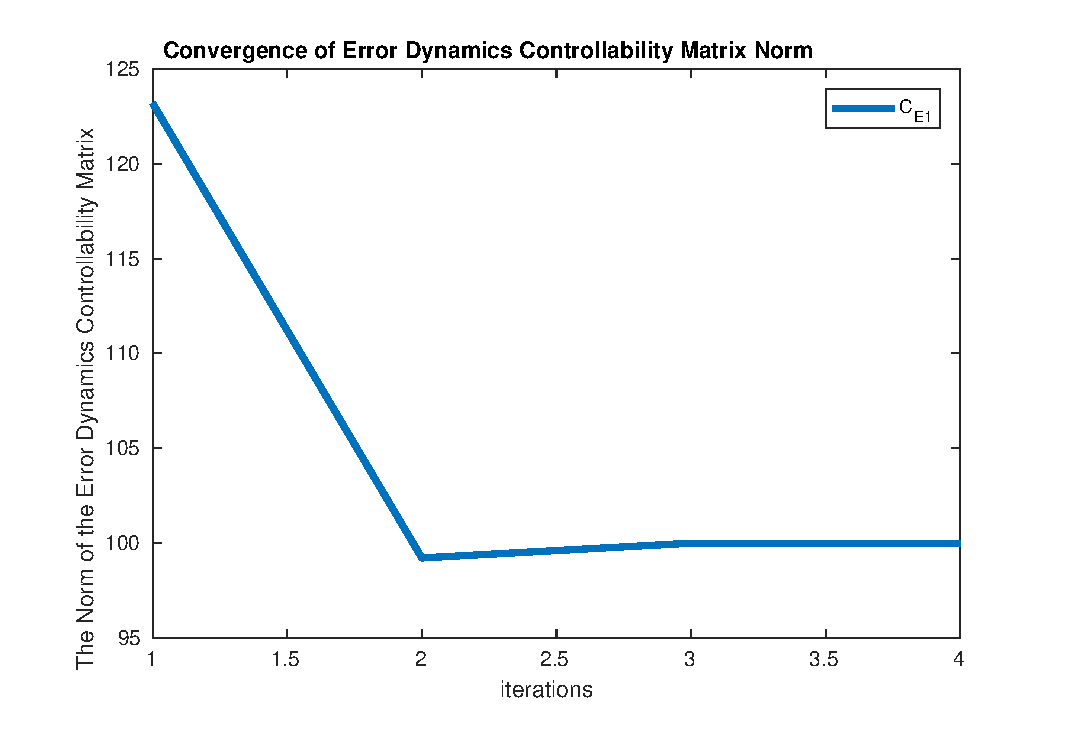
\includegraphics[width=0.7\textwidth]{ConNormTT.eps}
\caption{Convergence of error dynamics controllability matrix norm (6 thrusters, train and test)}	
\label{FIG:ConNormTT}
\end{figure}

%%%%%%%%%%%%%%%%%%%%%%%%%%%%%%%%%%%%%%%%%%%%%%%%%%%%%%%%%%%%%%%%%%%%%%%%%%%%%%%%%
\begin{figure}
\centering
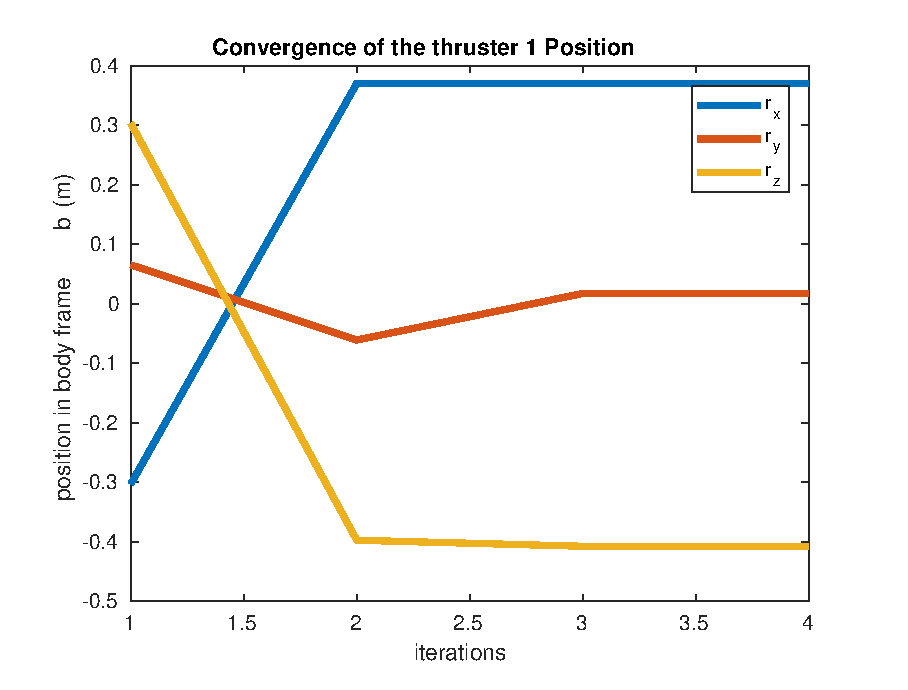
\includegraphics[width=0.45\textwidth]{ConThruster1PosTT.eps}
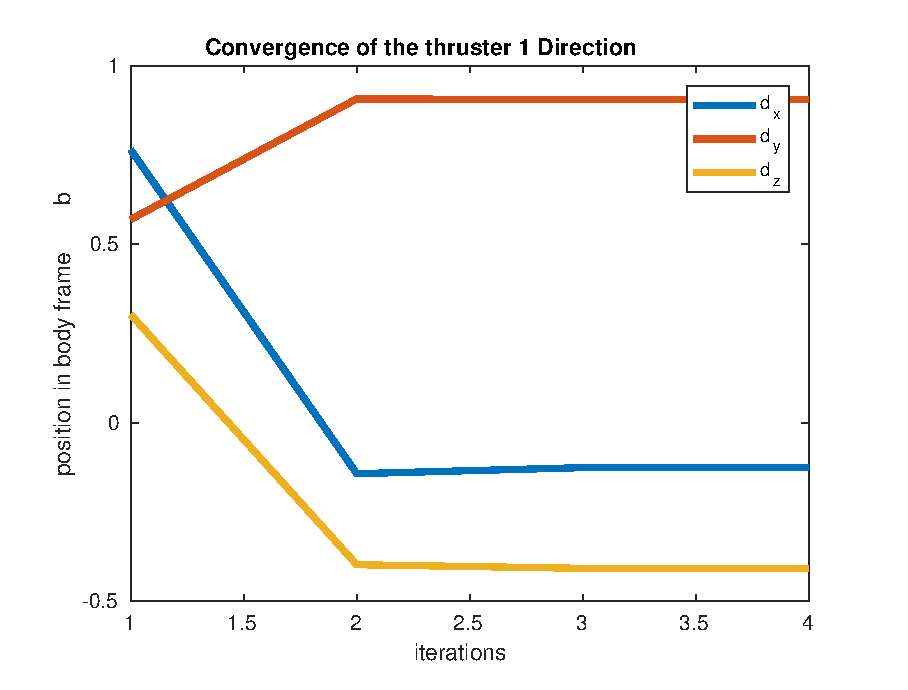
\includegraphics[width=0.45\textwidth]{ConThruster1DirTT.eps}
\caption{Convergence of position and direction of thruster 1 (6 thrusters, train and test)}	
\label{FIG:ConThruster1TT}
\end{figure}
\begin{figure}
\centering
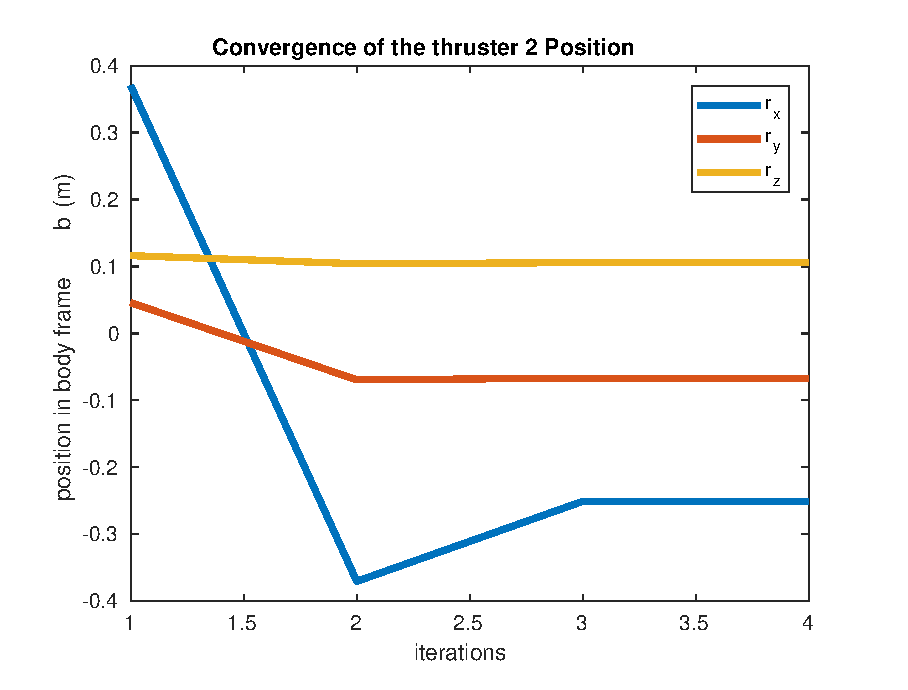
\includegraphics[width=0.45\textwidth]{ConThruster2PosTT.eps}
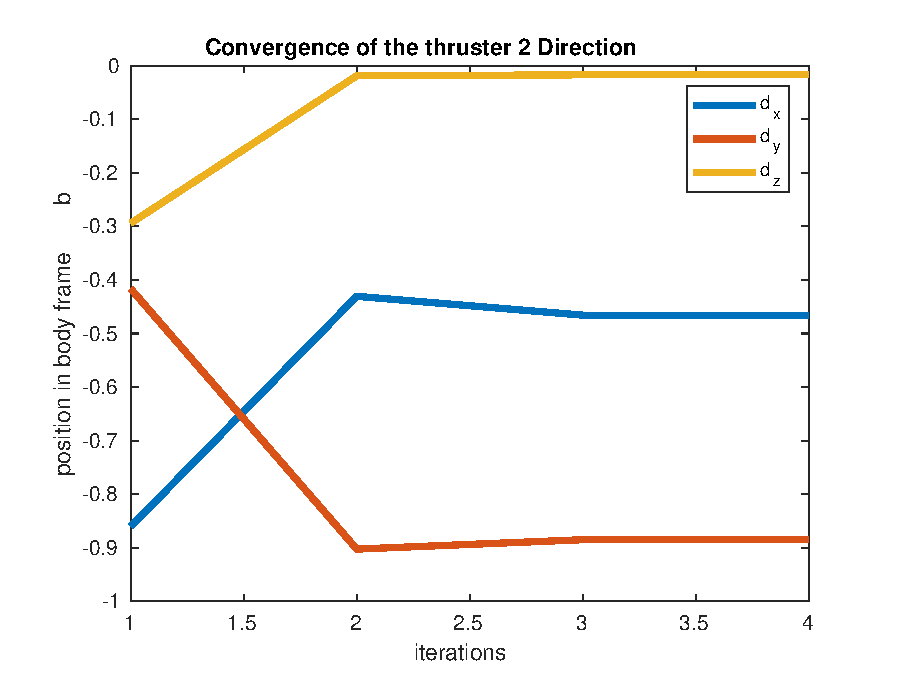
\includegraphics[width=0.45\textwidth]{ConThruster2DirTT.eps}
\caption{Convergence of position and direction of thruster 2 (6 thrusters, train and test)}	
\label{FIG:ConThruster2TT}
\end{figure}
\begin{figure}
\centering
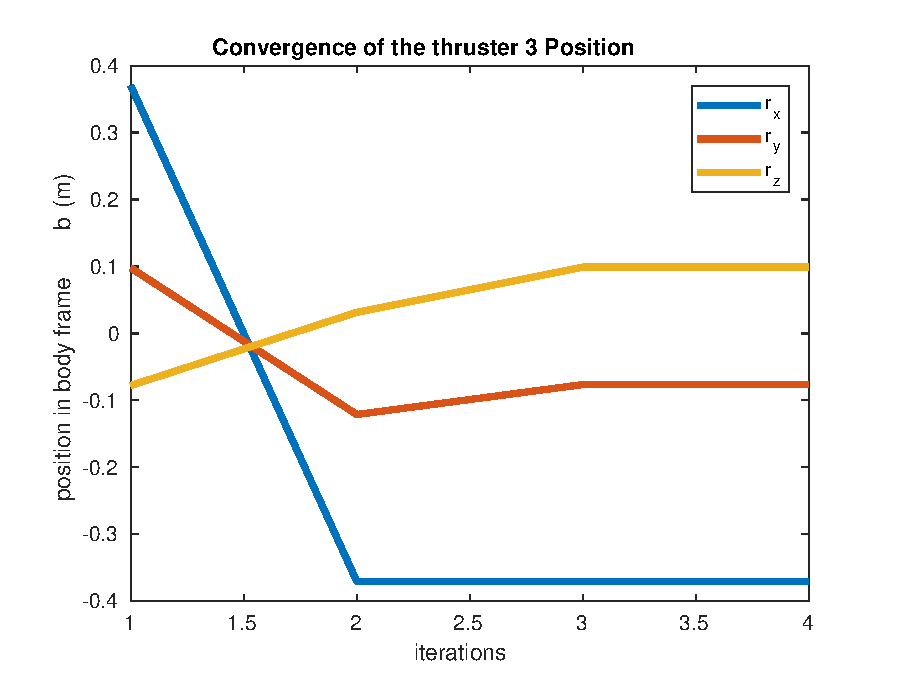
\includegraphics[width=0.45\textwidth]{ConThruster3PosTT.eps}
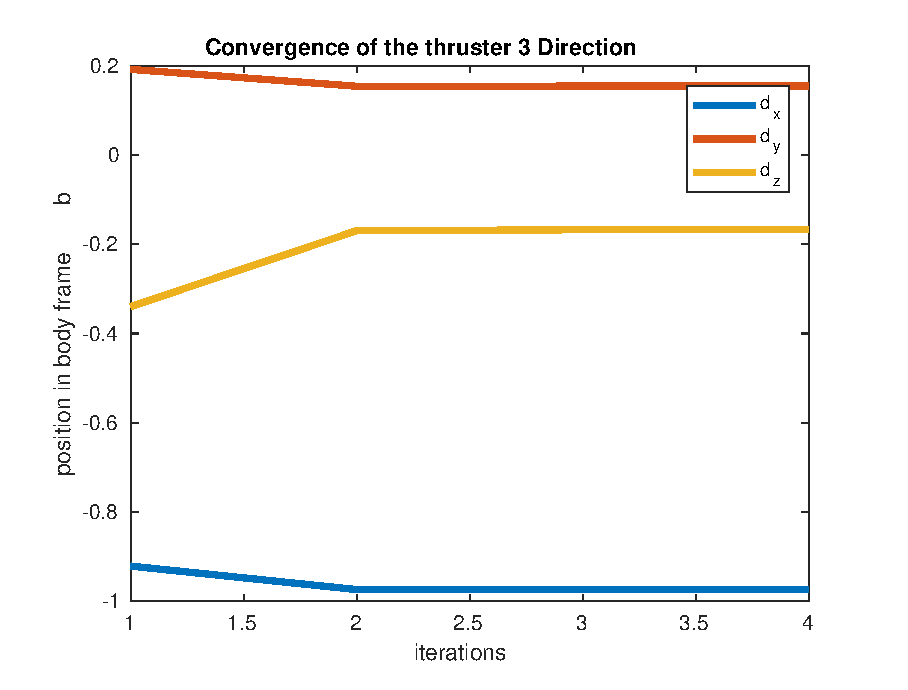
\includegraphics[width=0.45\textwidth]{ConThruster3DirTT.eps}
\caption{Convergence of position and direction of thruster 3 (6 thrusters, train and test)}	
\label{FIG:ConThruster3TT}
\end{figure}
\begin{figure}
\centering
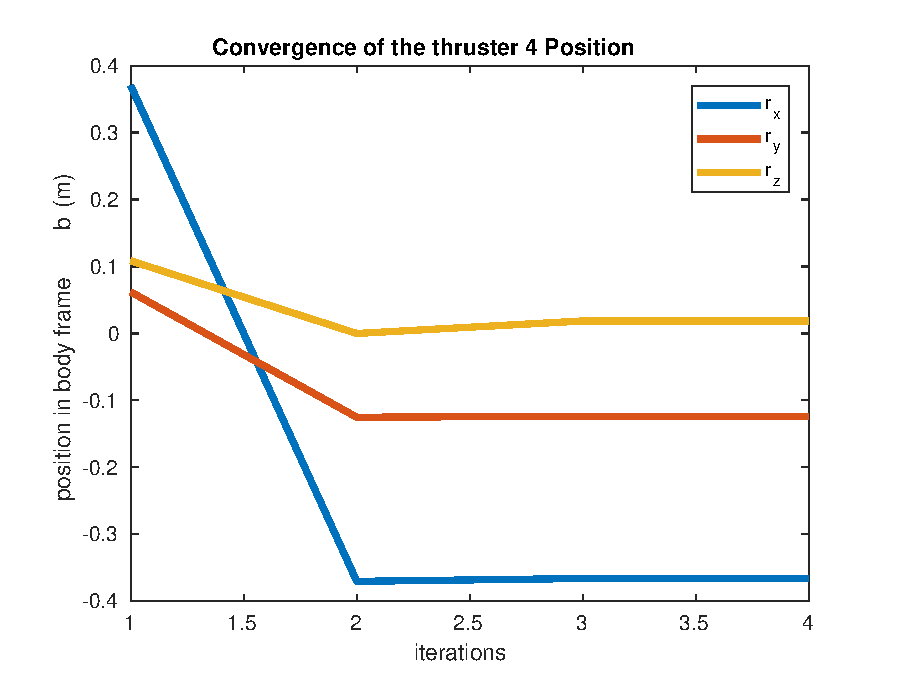
\includegraphics[width=0.45\textwidth]{ConThruster4PosTT.eps}
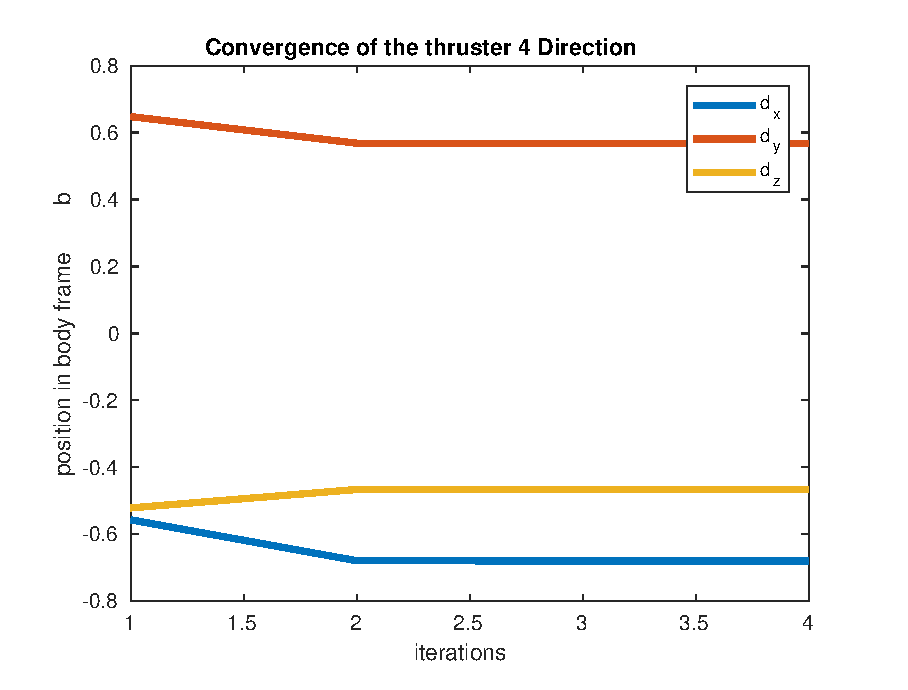
\includegraphics[width=0.45\textwidth]{ConThruster4DirTT.eps}
\caption{Convergence of position and direction of thruster 4 (6 thrusters, train and test)}	
\label{FIG:ConThruster4TT}
\end{figure}
\begin{figure}
\centering
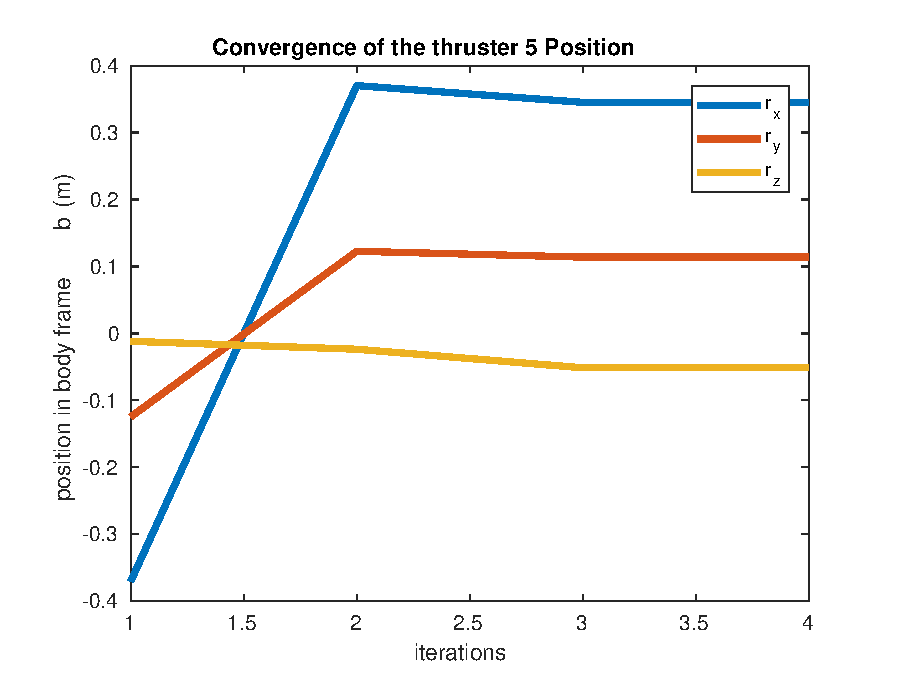
\includegraphics[width=0.45\textwidth]{ConThruster5PosTT.eps}
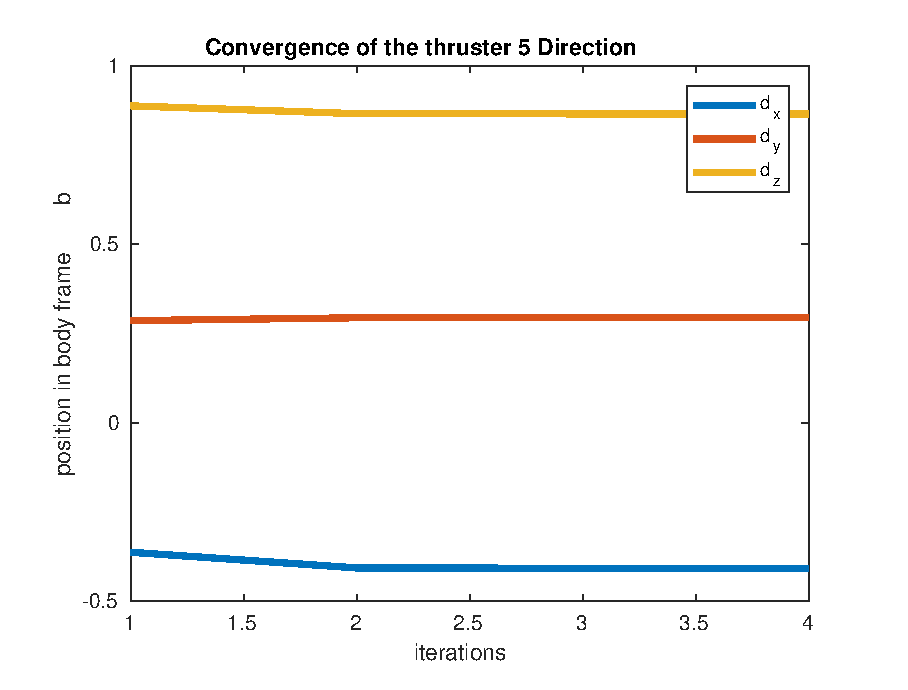
\includegraphics[width=0.45\textwidth]{ConThruster5DirTT.eps}
\caption{Convergence of position and direction of thruster 5 (6 thrusters, train and test)}	
\label{FIG:ConThruster5TT}
\end{figure}
\begin{figure}
\centering
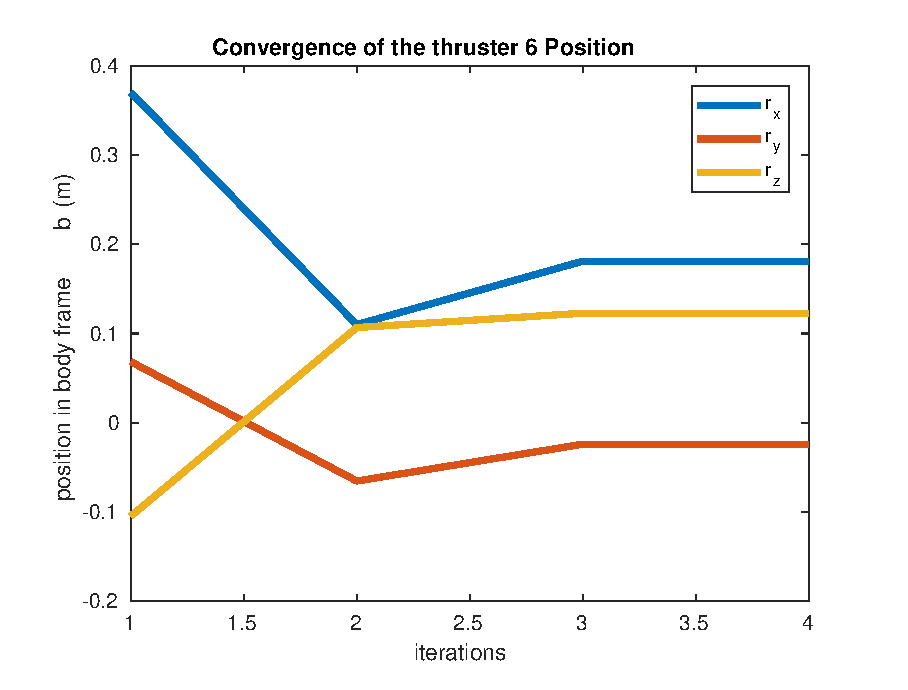
\includegraphics[width=0.45\textwidth]{ConThruster6PosTT.eps}
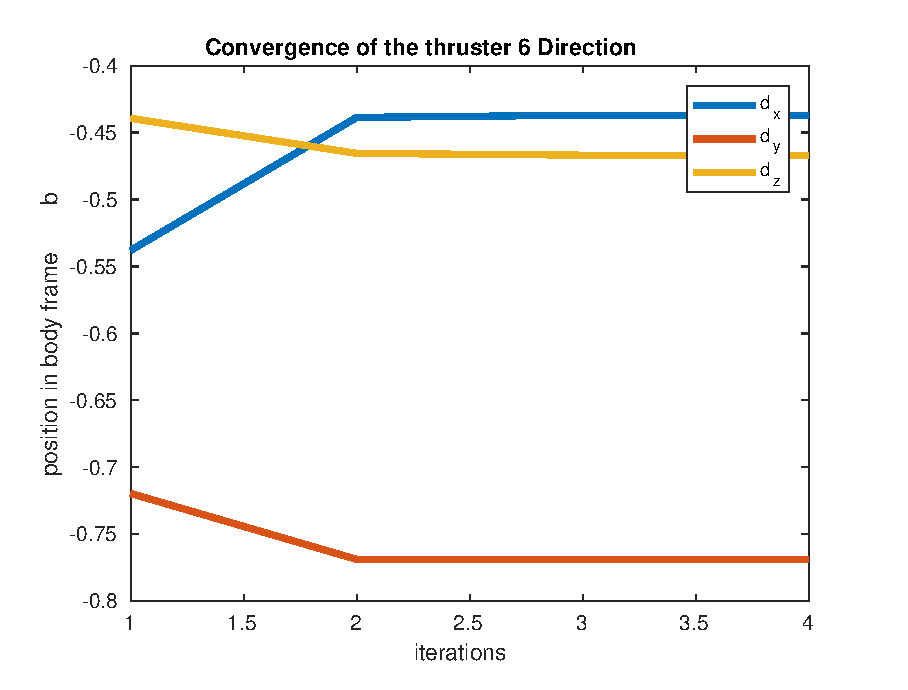
\includegraphics[width=0.45\textwidth]{ConThruster6DirTT.eps}
\caption{Convergence of position and direction of thruster 6 (6 thrusters, train and test)}	
\label{FIG:ConThruster6TT}
\end{figure}

\begin{figure}
\center
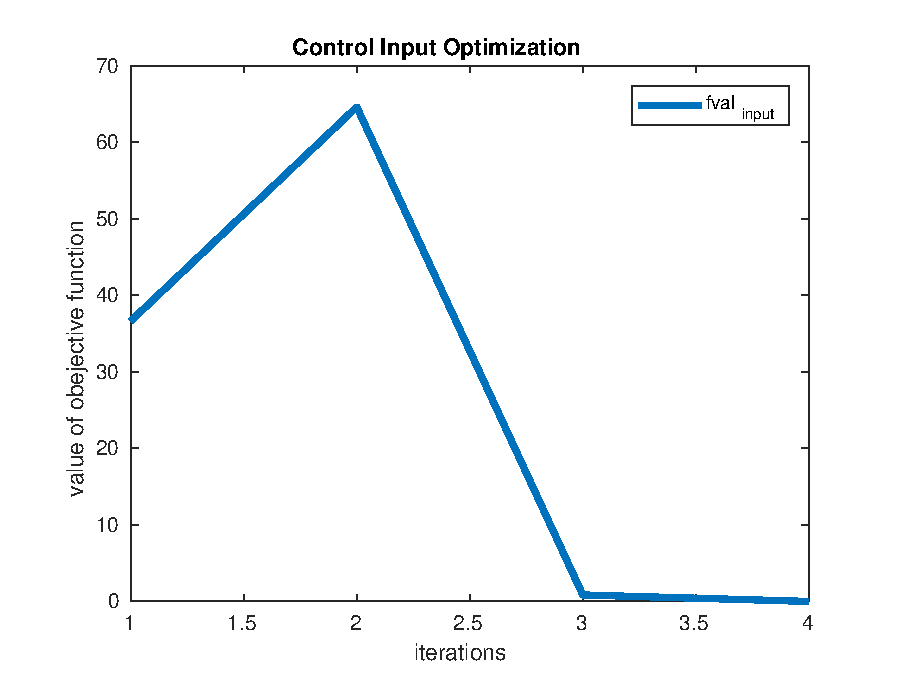
\includegraphics[width=0.49\textwidth]{ConInputTT.eps}
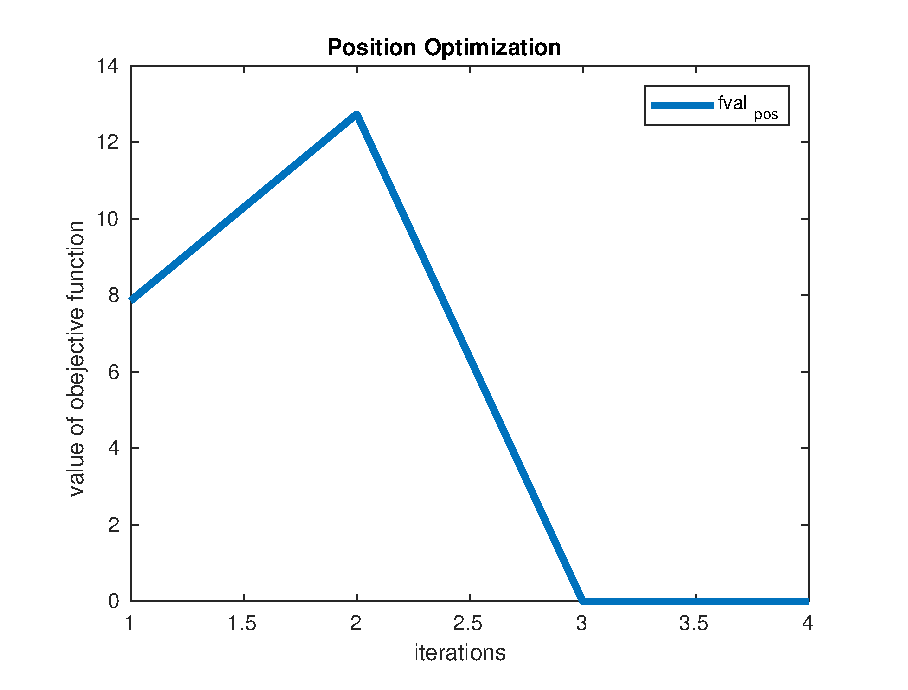
\includegraphics[width=0.49\textwidth]{ConPosTT.eps}
\caption{Value of objective function (6 thrusters, train and test)}	
\label{FIG:ConInputPosTT}
\end{figure}

\newpage
It is notable that the control input optimization error $fval_{input}$ and the position optimization error $fval_{pos}$ can be minimized to zero, which is not achievable for optimization in terms of seven trim trajectories. It is easy to find a actuator geometric configuration so that they can generate the desired trim input $\vec{\tau}_{\mathcal{T}}$ under saturation constraints for just one trim trajectory. However, when the desired trim trajectory segments increase to seven, 
a geometric configuration that is able to generate the desired seven trim generalized forces $\vec{\tau}_{d,\mathcal{T}_{1}}, \cdots, \vec{\tau}_{d,\mathcal{T}_{7}}$ under consideration of the actuator capability could not be found by our optimization algorithm.





\newpage

As illustrated in~\ref{FIG:TrackUnsatTT}, the trained robot from the first trim trajectory segment track both trim paths perfectly when the capability of the thrusters are not taken into consideration. The Figure~\ref{FIG:TrackSatTT} depicts the tracking performance when we specify the maximal and minimal thrust of the thrusters as $[-35,40]$ N. The tracking deviation from the desired train trim trajectory is bigger than that from the test trim trajectory due to its higher trim speed and yaw rate.

\begin{figure}
\centering
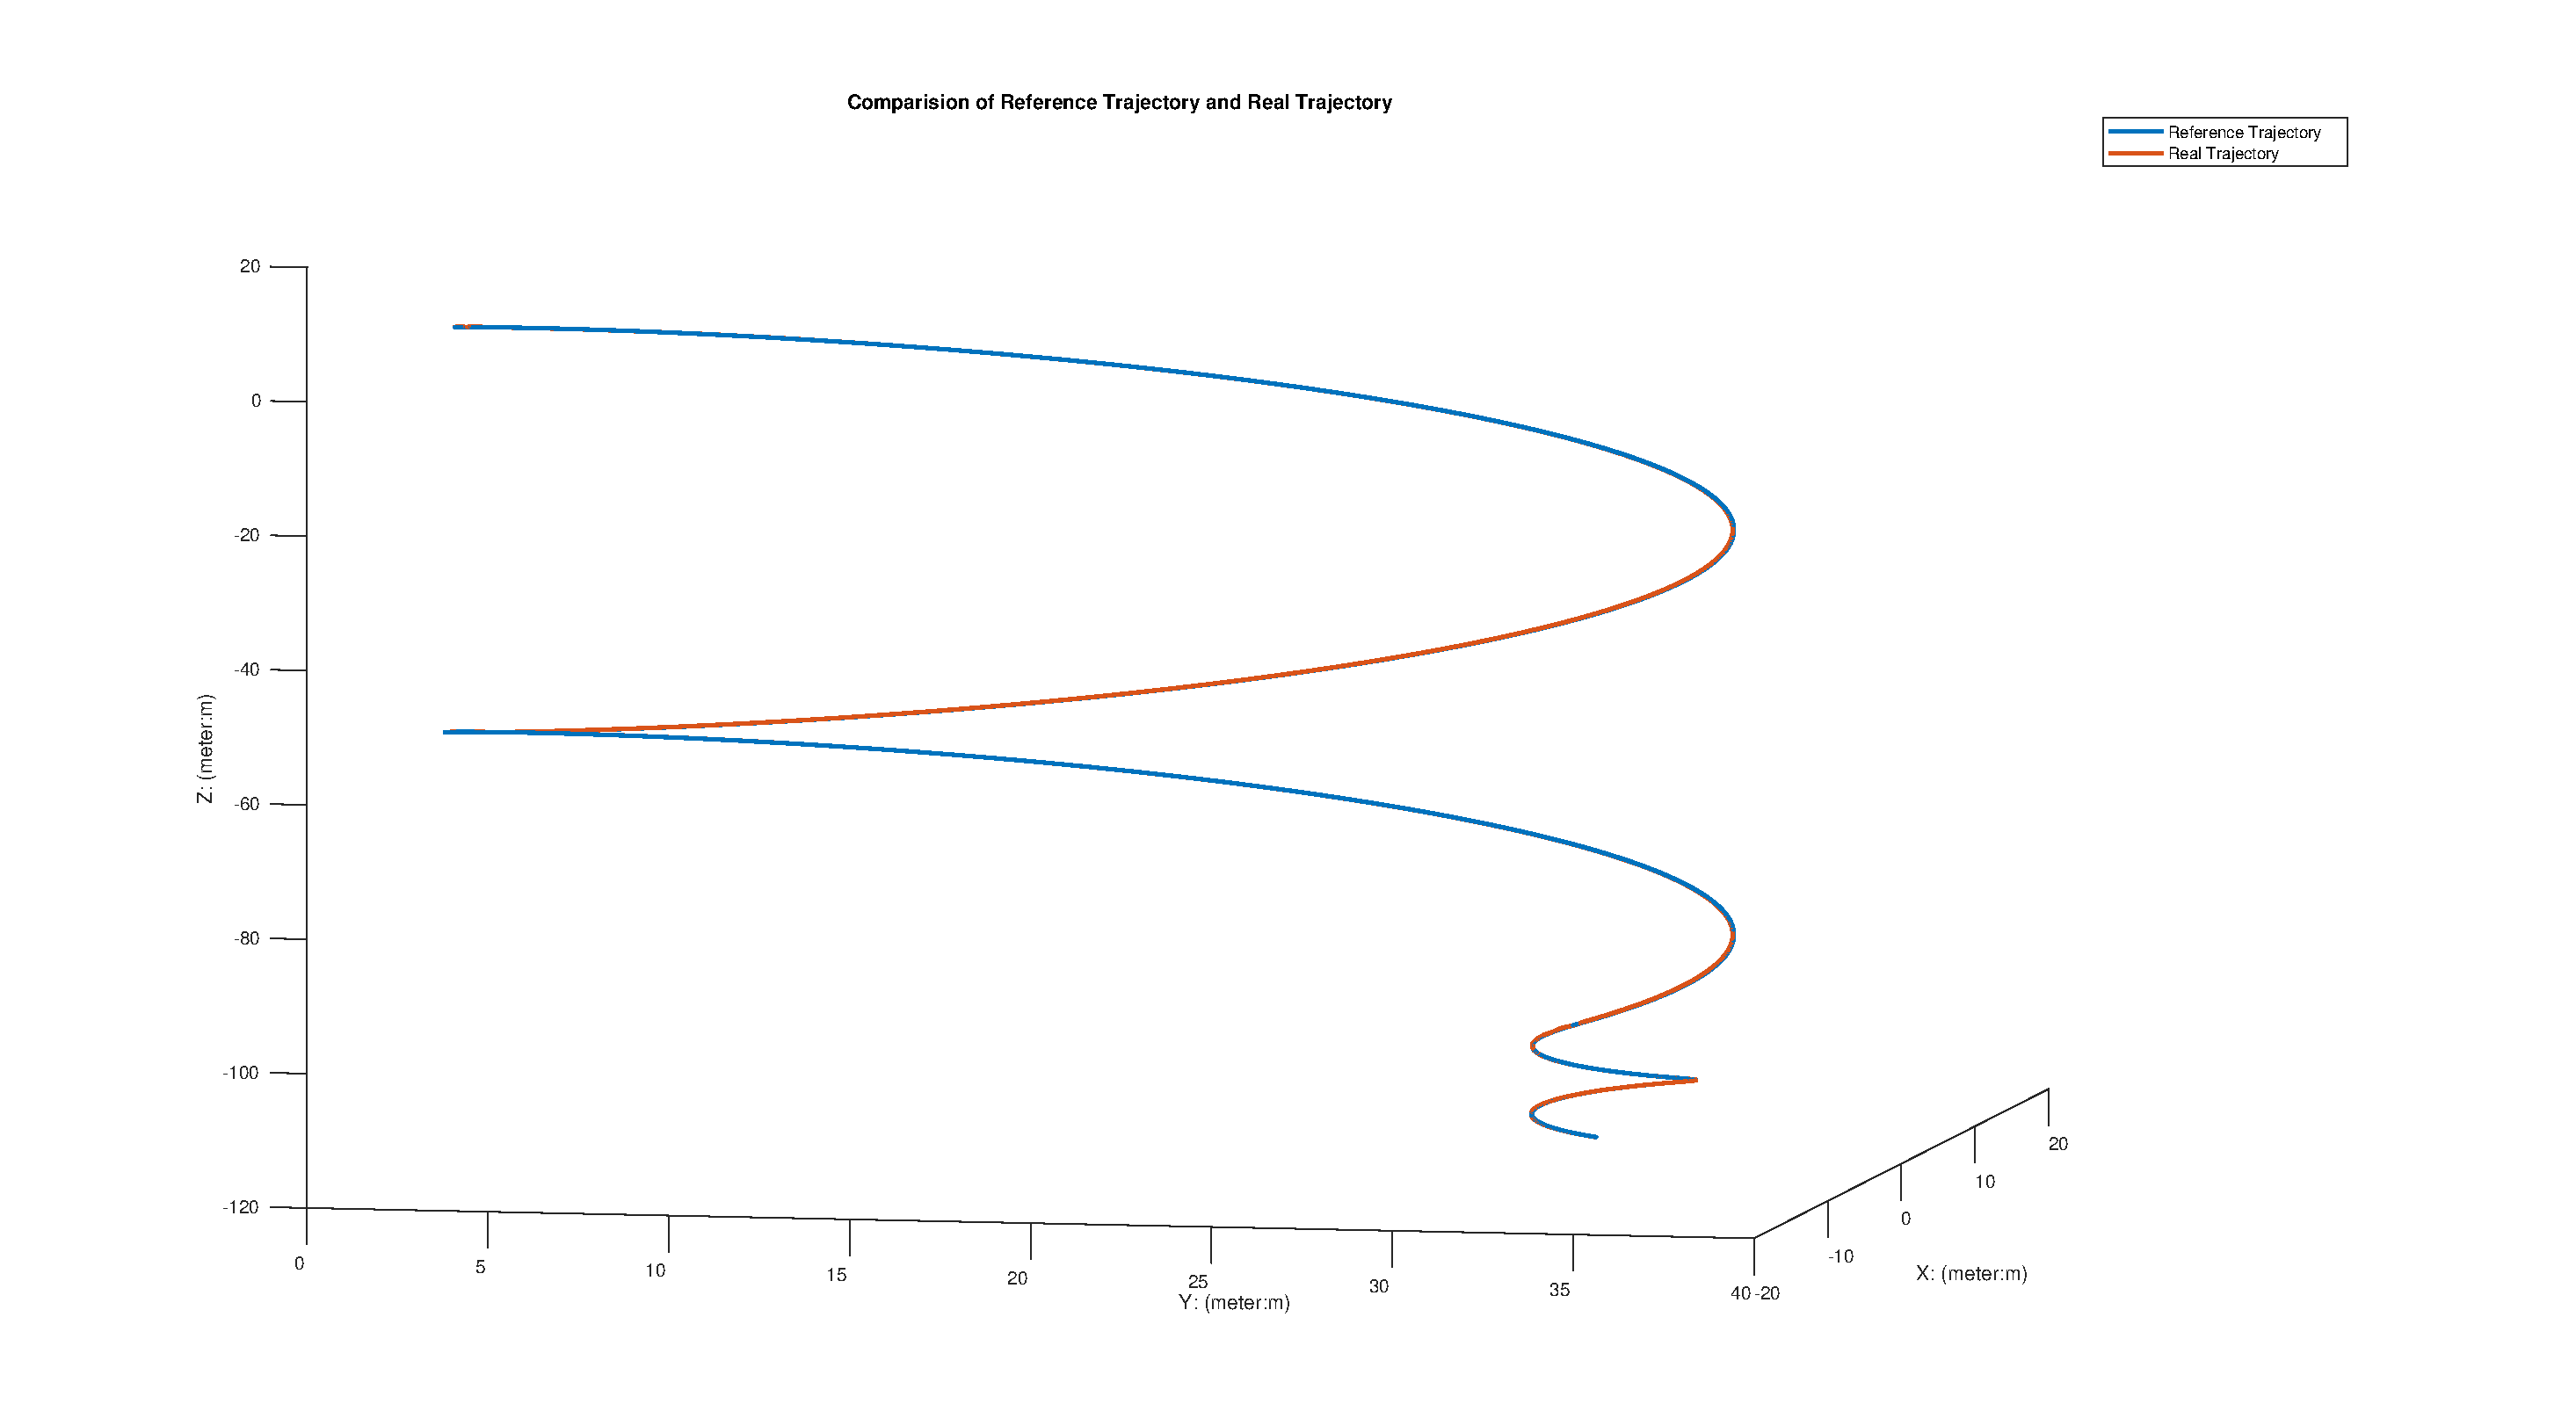
\includegraphics[width=\textwidth]{TrackUnsatTT.eps}
\caption{Comparison of desired trajectory and real trajectory (6 thrusters, no actuator saturation, train and test)}	
\label{FIG:TrackUnsatTT}
\end{figure}
\begin{figure}[h]
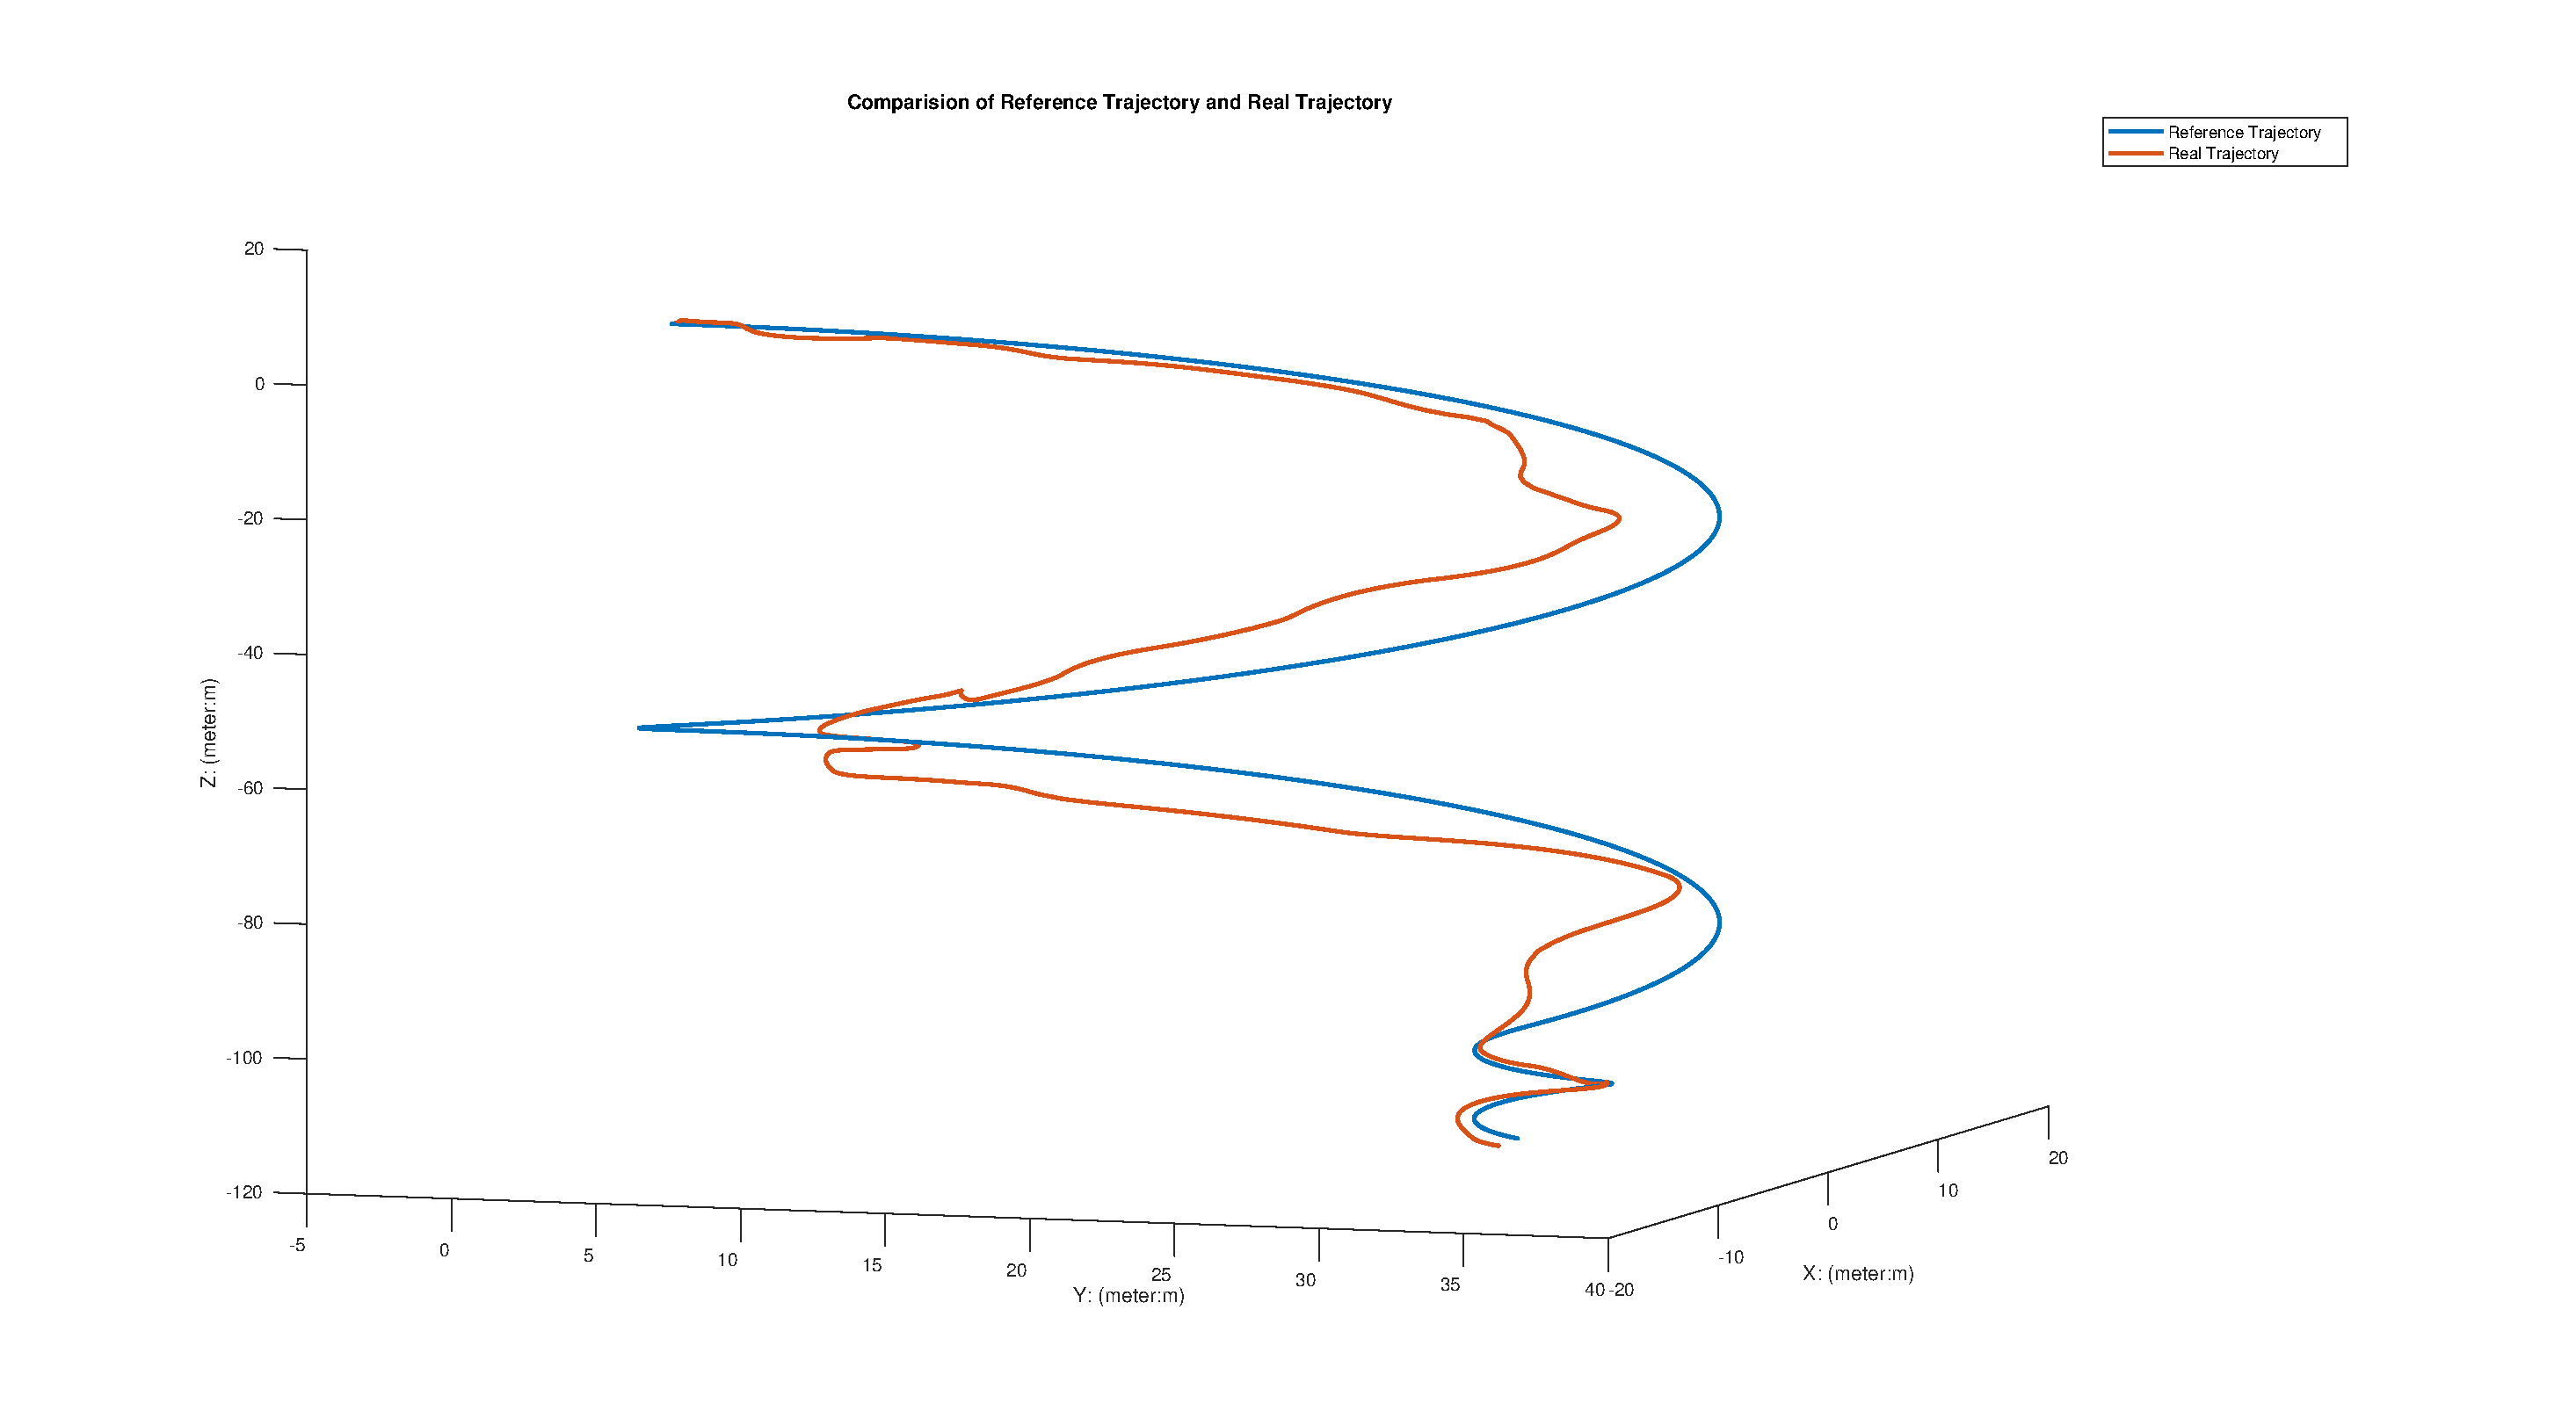
\includegraphics[width=\textwidth]{TrackSatTT.eps}
\caption{Comparison of desired trajectory and real trajectory (6 thrusters, with actuator saturation, train and test)}	
\label{FIG:TrackSatTT}
\end{figure}
%%%%%%%%%%%%%%%%%%%%%%%%%%%%%%%%%%%%%%%%%%%%%%%%%%%%%%%%%%%%%%%%%%%%%%%%%%%%%%%%%%
\section{Simulation for 4 Fins and 2 Thrusters} 
Compared with pure thrusters configuration, the placement of fins deserves further study since they are trajectory dependent. Not only the geometric variables concerning fins but also the trim specifications will contribute to the generated generalized force. Assume that the robot now has 4 fins and 2 thrusters to control its motion. In this case, we also set $\epsilon=0.001\times\dfrac{1}{7}\sum_{j=1}^{7}||\emph{\textbf{C}}_{E,j}^{1}||$.
%%%%%%%%%%%%%%%%%%%%%%%%%%%%%%%%%%%%%%%%%%%%%%%%%%%%%%%%%%%%%%%%%%%%%%%%%%%%%

As depicted in Figures~\ref{FIG:GeoVisualFinThruster21} and~\ref{FIG:GeoVisualFinThruster22}, the fins allocation in this case is quasi-symmetrical, two fins are located on the right front hull and other two are located on the left tail part of the hull. One thruster points to the right front side while other points to the left front side.  
\begin{figure}
\center
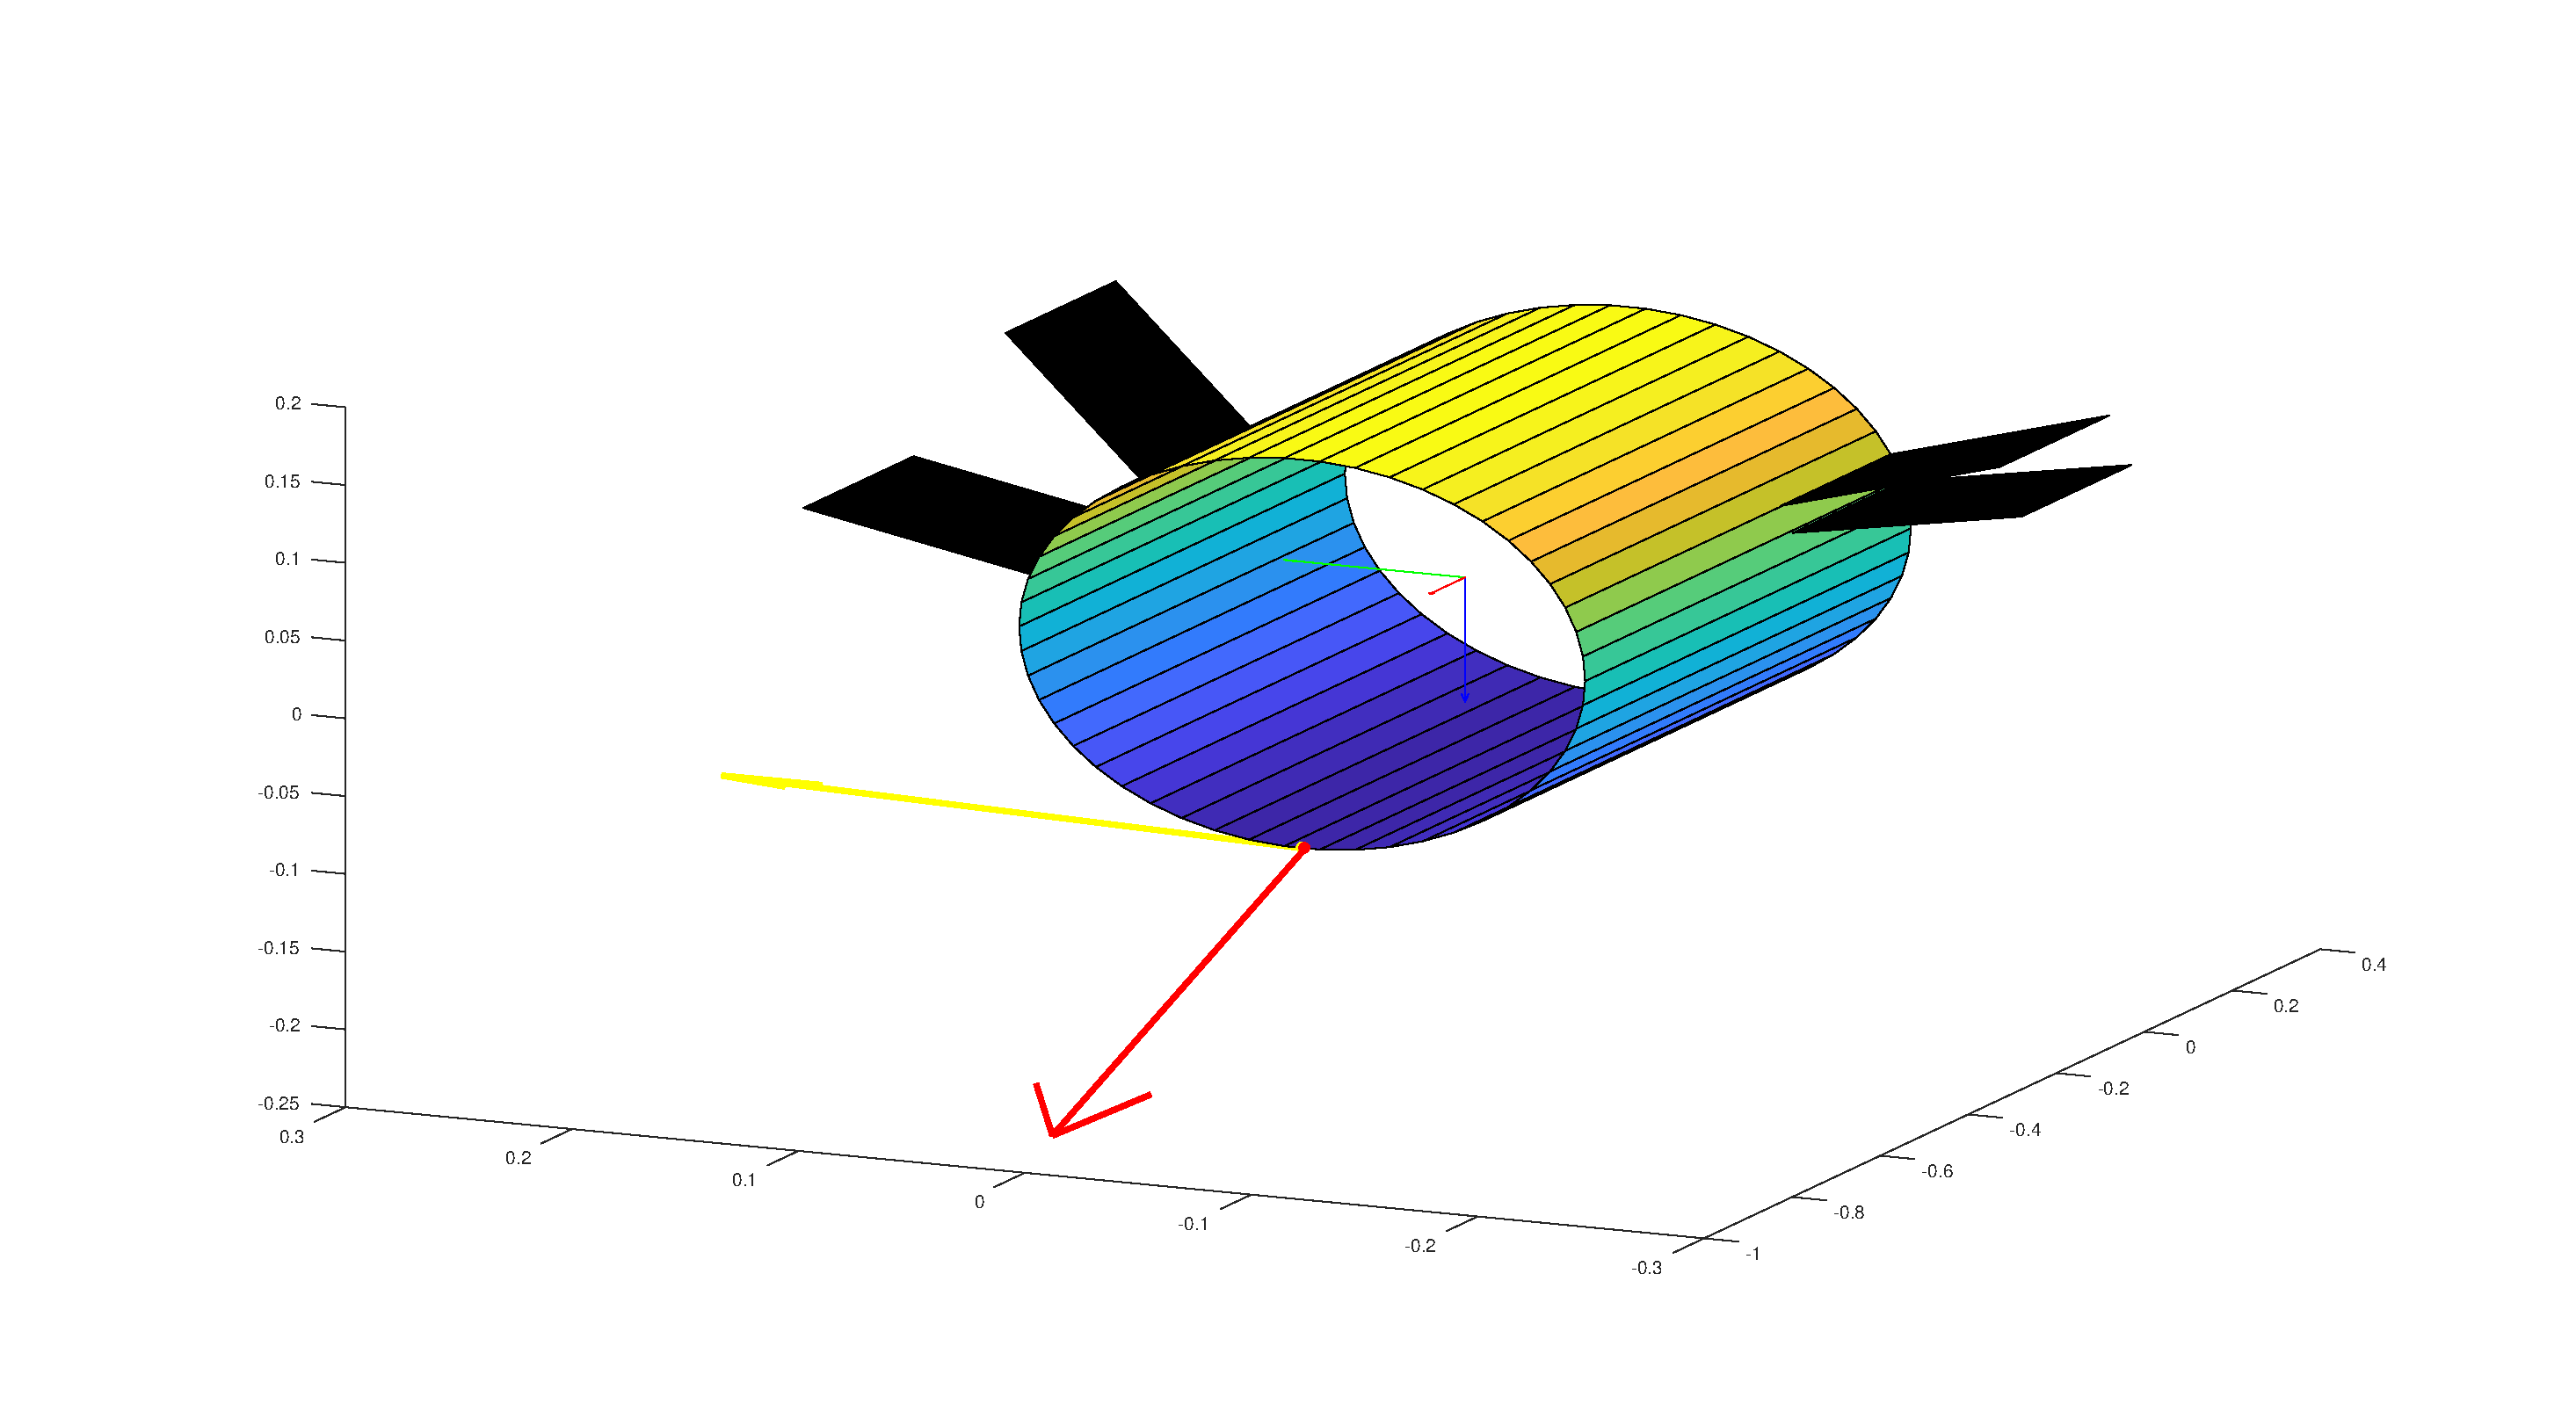
\includegraphics[width=0.9\textwidth]{GeoVisualFinThruster21.eps}
\caption{Visualization of optimization result (4 fins and 2 thrusters) perspective 1}	
\label{FIG:GeoVisualFinThruster21}
\end{figure}
\begin{figure}
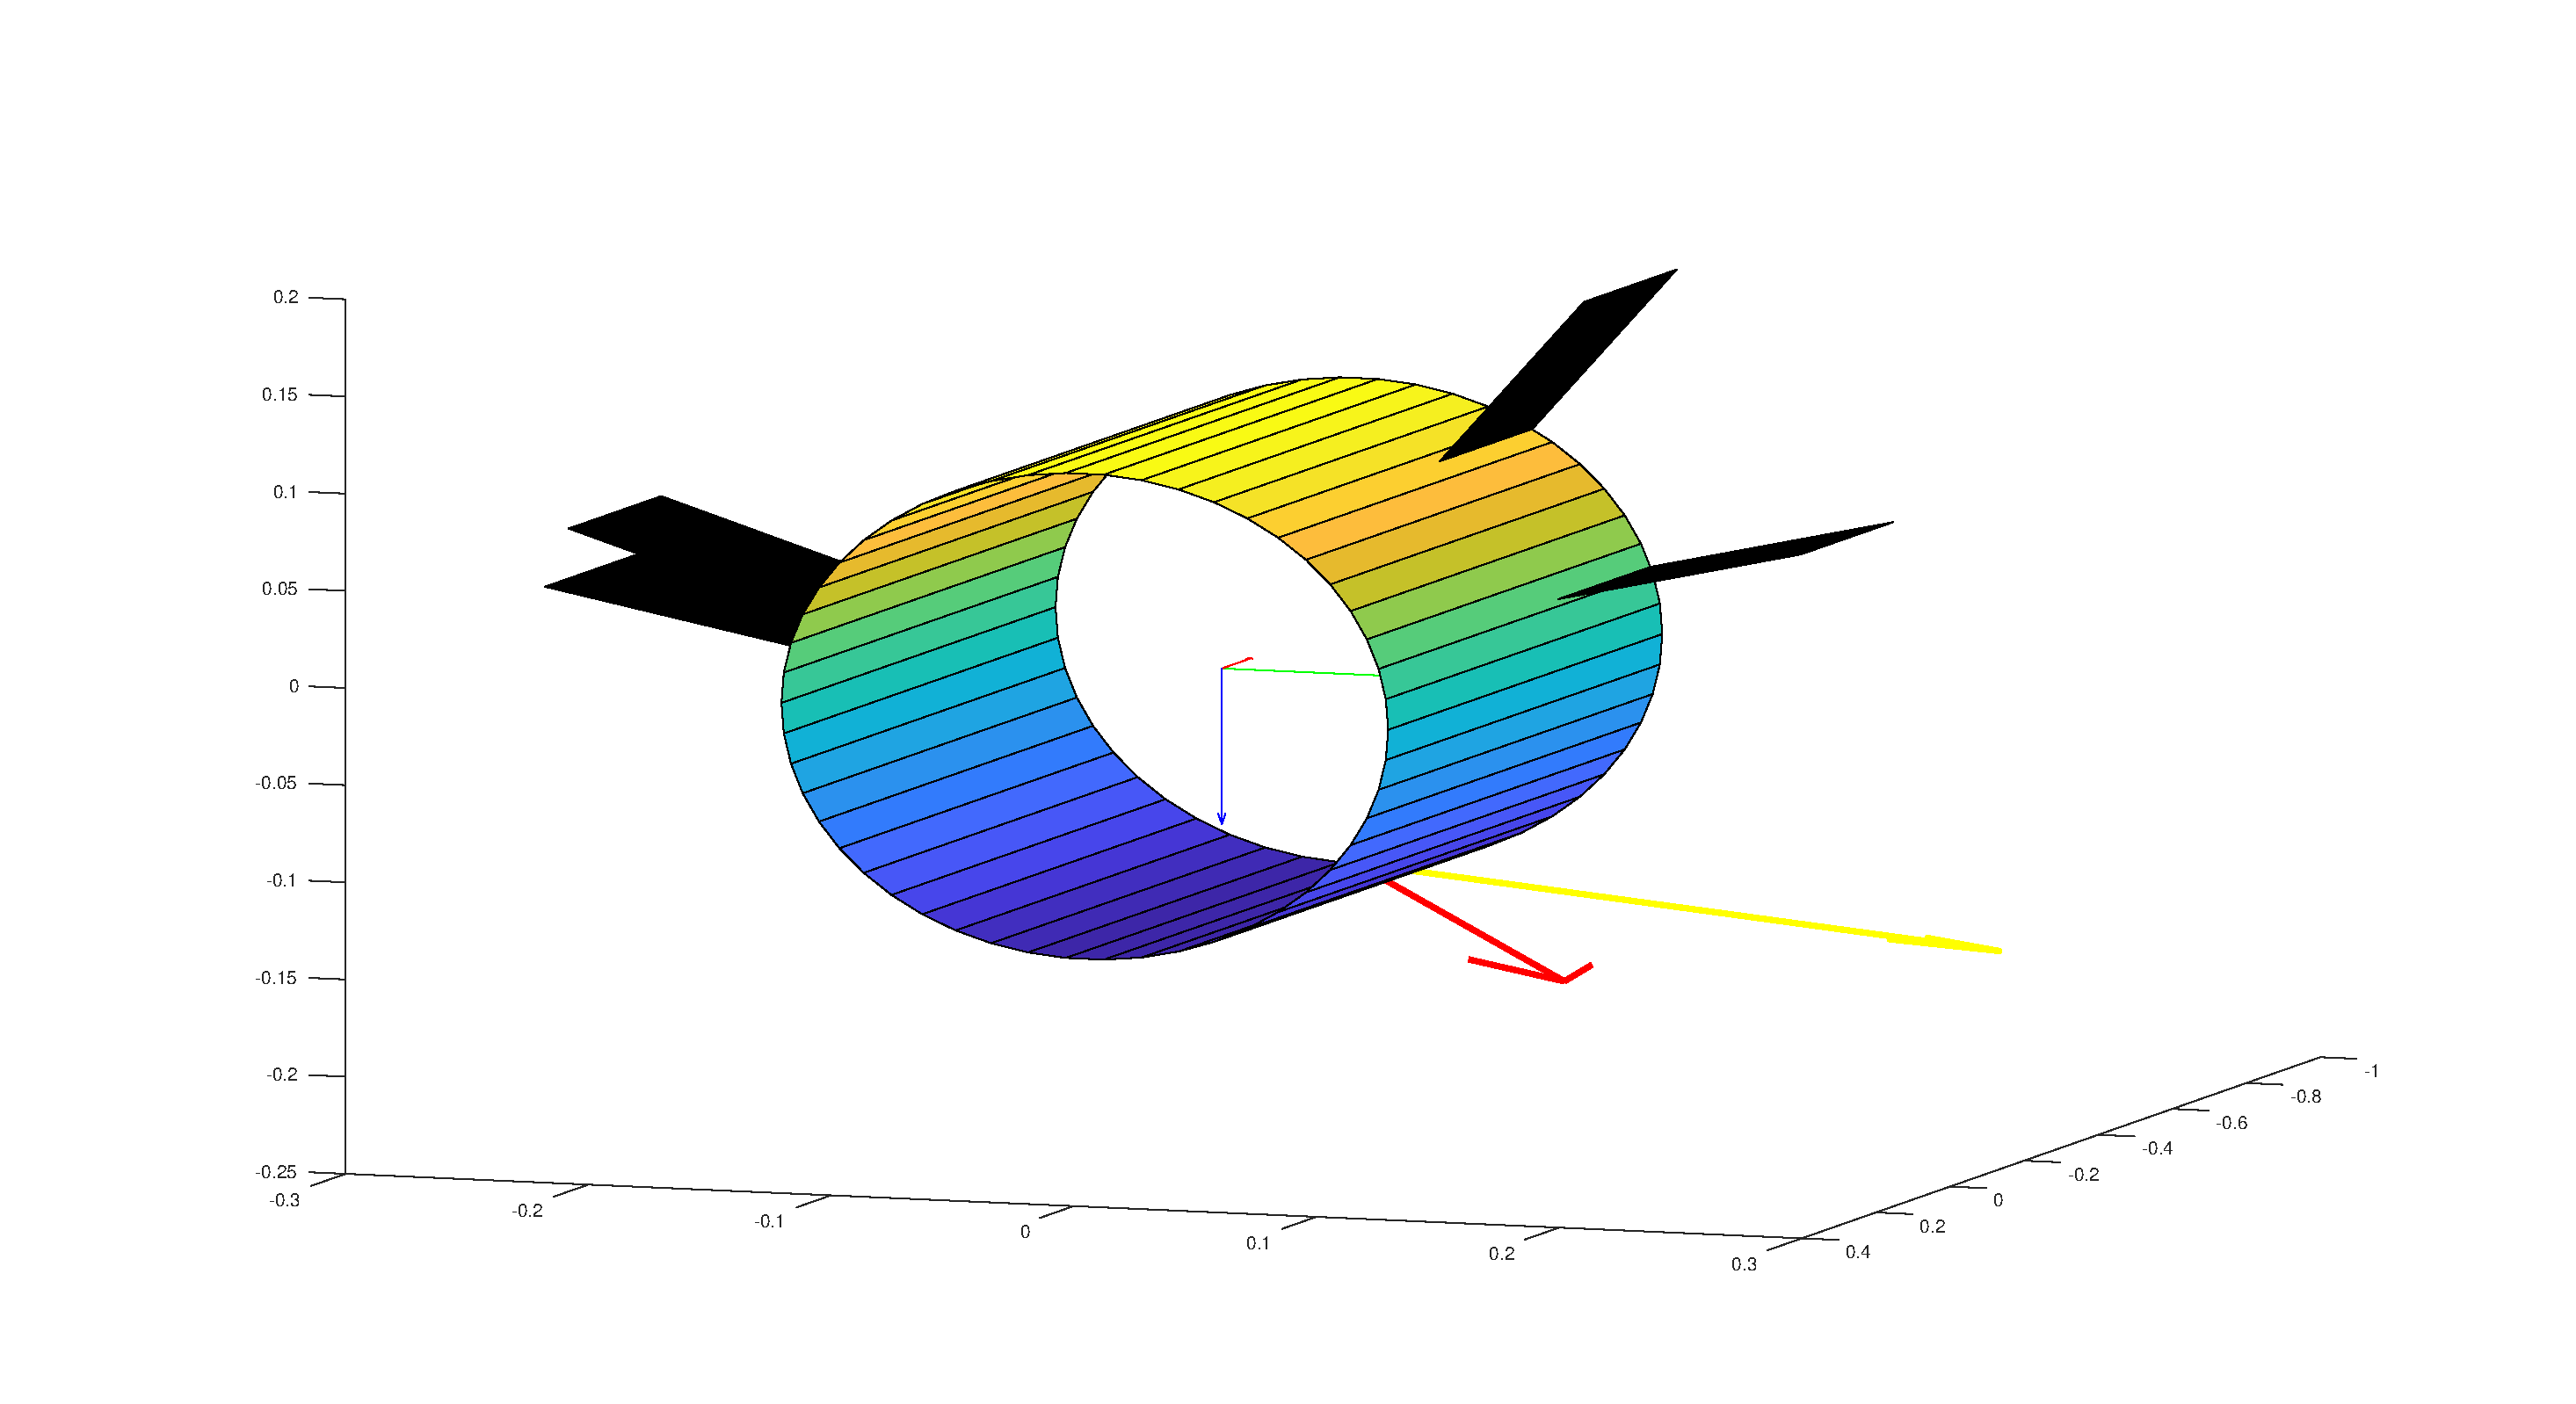
\includegraphics[width=\textwidth]{GeoVisualFinThruster22.eps}
\caption{Visualization of optimization result (4 fins and 2 thrusters) perspective 2}	
\label{FIG:GeoVisualFinThruster22}
\end{figure}
%%%%%%%%%%%%%%%%%%%%%%%%%%%%%%%%%%%%%%%%%%%%%%%%%%%%%%%%%%%%%%%%%%%%%%%%%%%%%%%%
From Figures~\ref{FIG:ConFin12},~\ref{FIG:ConFin22},~\ref{FIG:ConFin32} and~\ref{FIG:ConFin42}, we can see that the positions $x_{F,1}$, $x_{F,2}$, $x_{F,3}$ and $x_{F,4}$ stay constant after about 38 iterations, while the orientations keep on changing. It can be seen from Figures \ref{FIG:ConThruster12} and \ref{FIG:ConThruster22} that the positions and orientations of thruster 1 and thruster 2 converge after about 50 iterations. 
\begin{figure}
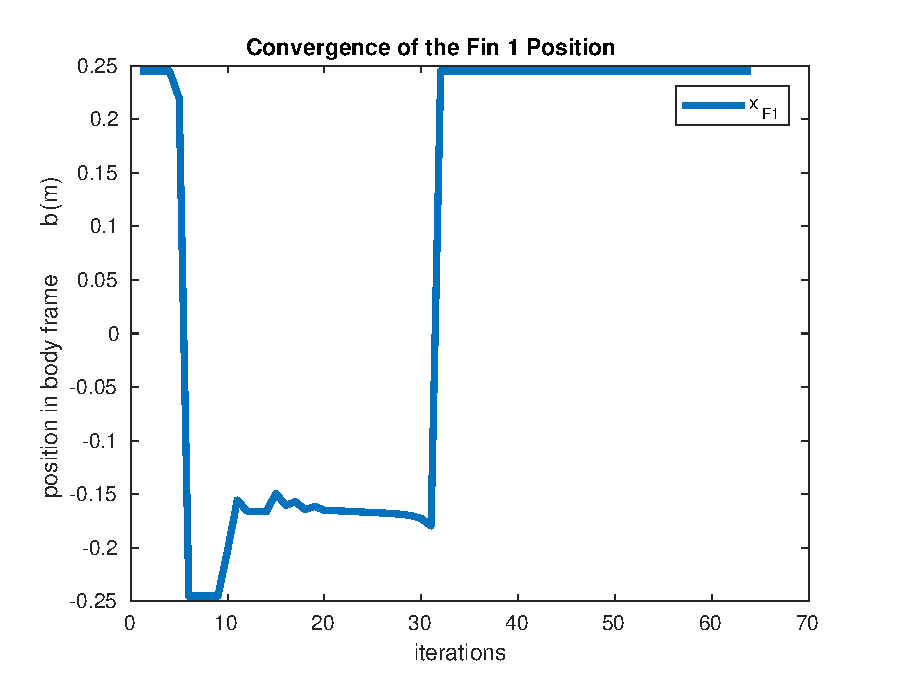
\includegraphics[width=0.5\textwidth]{ConFin1Pos2.eps}
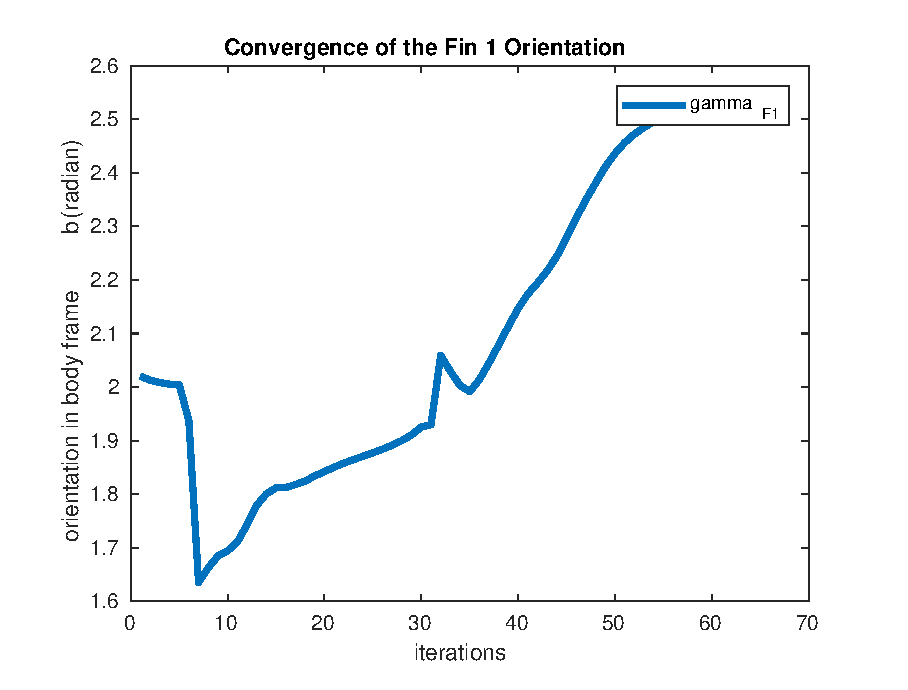
\includegraphics[width=0.5\textwidth]{ConFin1Orient2.eps}
\caption{Convergence of position and orientation of fin 1 (4 fins and 2 thrusters)}	
\label{FIG:ConFin12}
\end{figure}
\begin{figure}
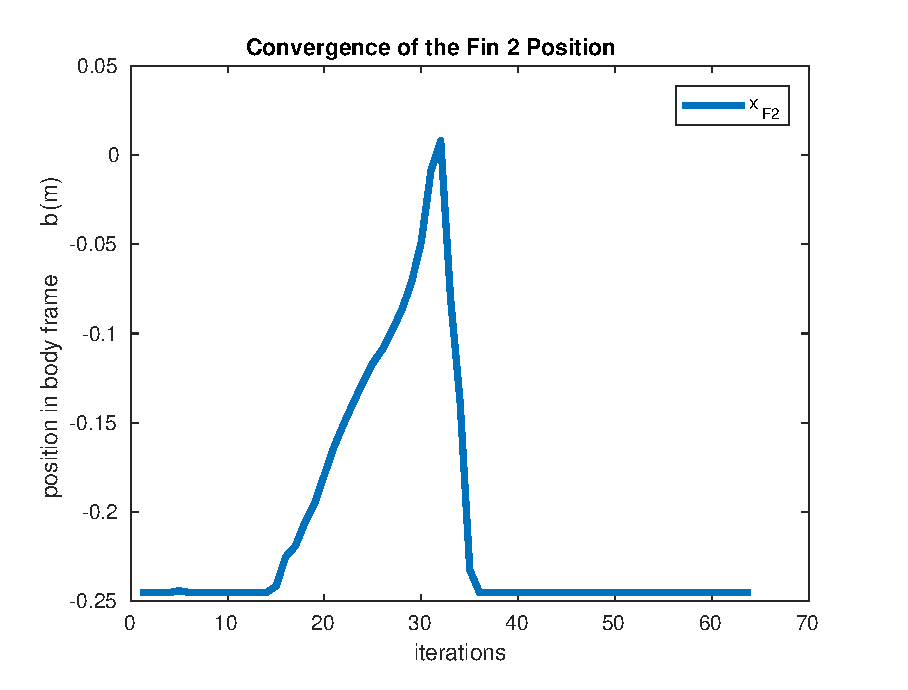
\includegraphics[width=0.5\textwidth]{ConFin2Pos2.eps}
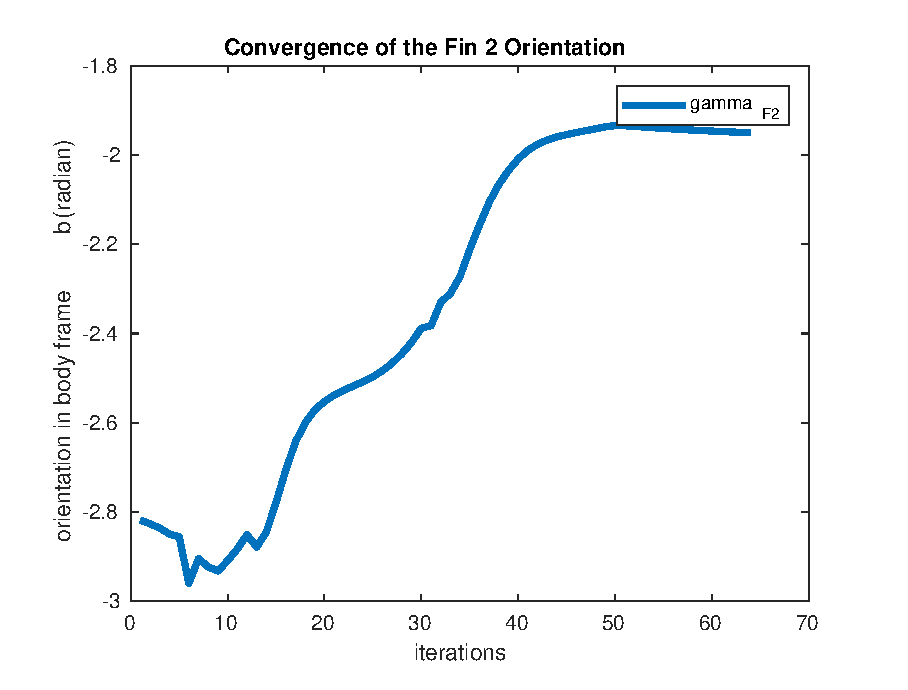
\includegraphics[width=0.5\textwidth]{ConFin2Orient2.eps}
\caption{Convergence of position and orientation of fin 2 (4 fins and 2 thrusters)}	
\label{FIG:ConFin22}
\end{figure}
\begin{figure}
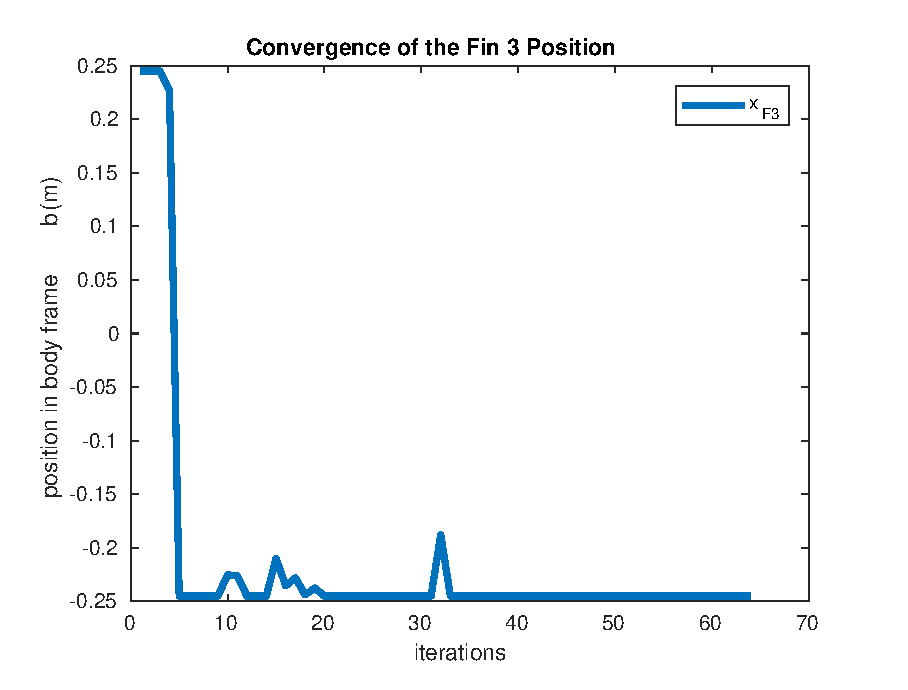
\includegraphics[width=0.5\textwidth]{ConFin3Pos2.eps}
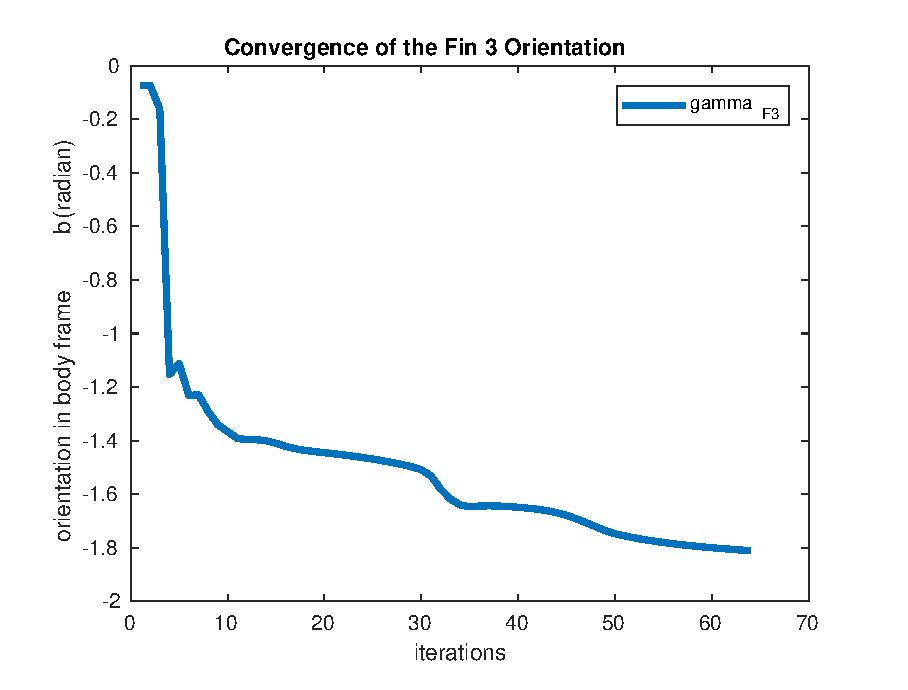
\includegraphics[width=0.5\textwidth]{ConFin3Orient2.eps}
\caption{Convergence of position and orientation of fin 3 (4 fins and 2 thrusters)}	
\label{FIG:ConFin32}
\end{figure}
\begin{figure}
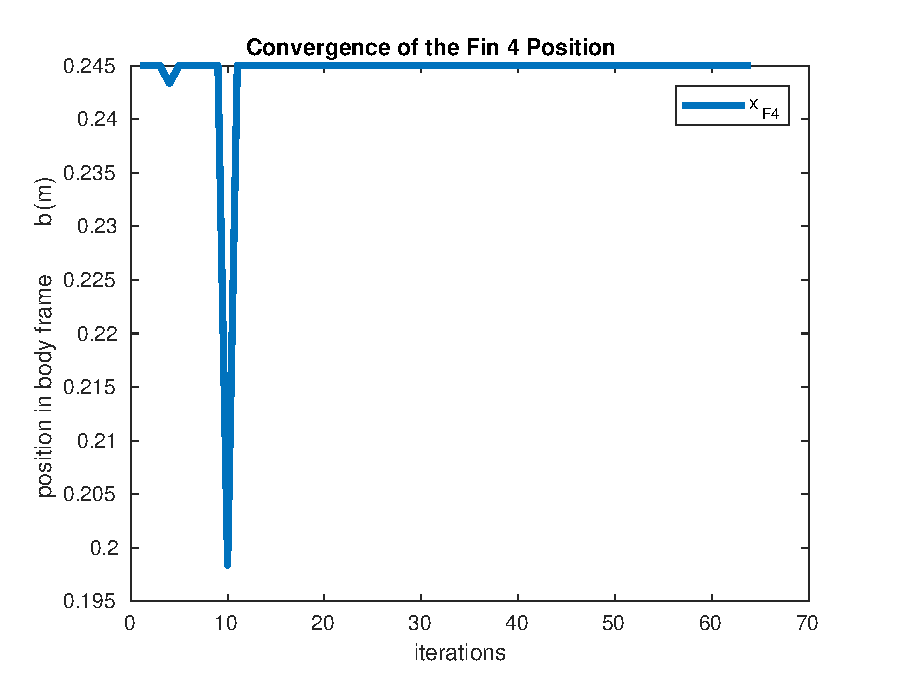
\includegraphics[width=0.5\textwidth]{ConFin4Pos2.eps}
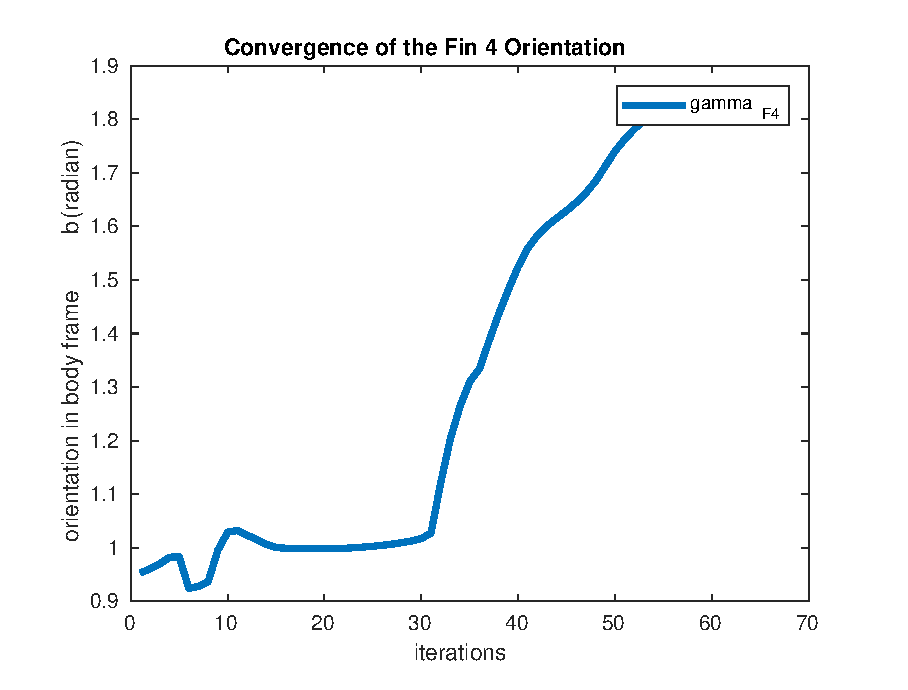
\includegraphics[width=0.5\textwidth]{ConFin4Orient2.eps}
\caption{Convergence of position and orientation of fin 4 (4 fins and 2 thrusters)}	
\label{FIG:ConFin42}
\end{figure}
\begin{figure}
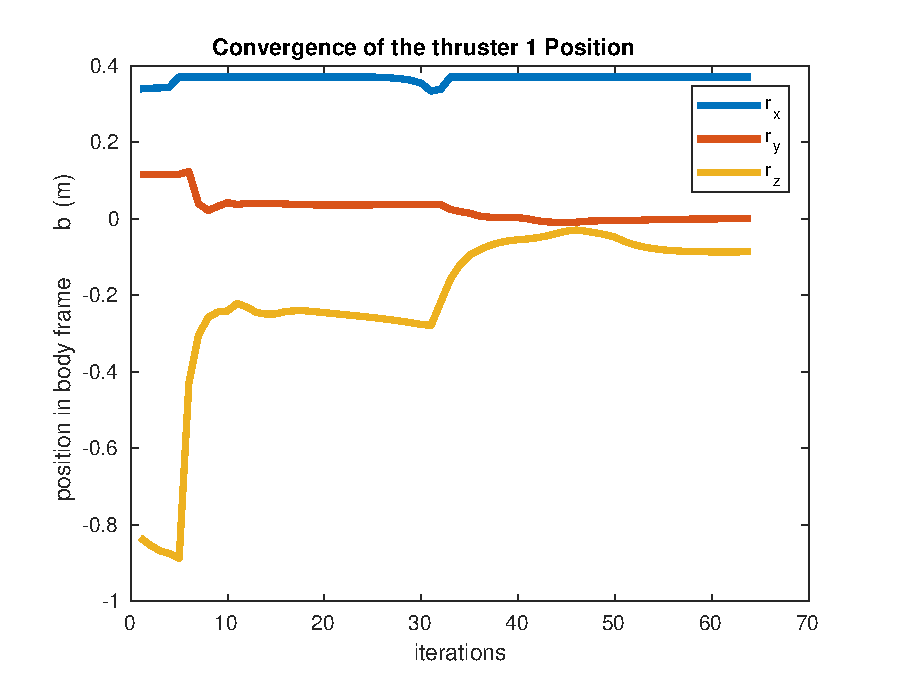
\includegraphics[width=0.5\textwidth]{ConThruster1Pos2.eps}
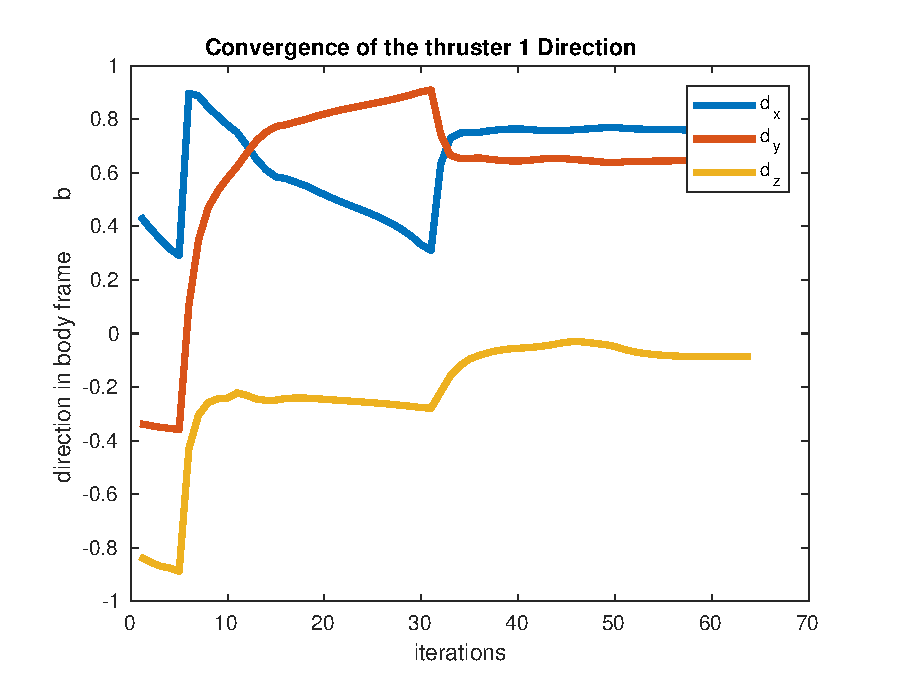
\includegraphics[width=0.5\textwidth]{ConThruster1Dir2.eps}
\caption{Convergence of position and direction of thruster 1 (4 fins and 2 thrusters)}	
\label{FIG:ConThruster12}
\end{figure}
\begin{figure}
\includegraphics[width=0.5\textwidth]{ConThruster2Pos2.eps}
\includegraphics[width=0.5\textwidth]{ConThruster2Dir2.eps}
\caption{Convergence of position and direction of thruster 2}	
\label{FIG:ConThruster22}
\end{figure}
\begin{figure}
\centering
\includegraphics[width=0.75\textwidth]{ConNorm2.eps}
\caption{Convergence of error dynamics controllability matrix norm (4 fins and 2 thrusters)}	
\label{FIG:ConNorm2}
\end{figure}
\newpage
%%%%%%%%%%%%%%%%%%%%%%%%%%%%%%%%%%%%%%%%%%%%%%%%%%%%%%%%%%%%%%%%%%%%%%%%%%%%%%%%%
The value of the control input objective function $fval_{input}$ increases at first and then falls down sharply from the 5-th iteration to the 10-th iteration. Afterwards, it restarts to increase until the 30-th iteration and then falls down again. The position optimization objective function $fval_{pos}$ rises sharply in the beginning but decreases quickly to about 50. 
\begin{figure}
\center
\includegraphics[width=0.49\textwidth]{ConInput2.eps}
\includegraphics[width=0.49\textwidth]{ConPos2.eps}
\caption{Value of objective function (4 fins and 2 thrusters)}	
\label{FIG:ConPosInput2}
\end{figure}
\newpage
%%%%%%%%%%%%%%%%%%%%%%%%%%%%%%%%%%%%%%%%%%%%%%%%%%%%%%%%%%%%%%%%%%%%%%%%%%
We use the state and input cost matrices in Table~\ref{table:QParameters} and Table~\ref{table:RParameters for 4 fins and 2 thrusters} to design the switched LQR controller. Note that in this case smaller input weighting matrices are chosen meaning larger control inputs are needed to track the desired trajectory.  
\begin{table}
\centering
\small
\caption{Input cost matrices for 4 fins and 2 thrusters}
\begin{tabular}{| c | c | c | c | p{0.5cm} |}
\hline
Index&$\mathcal{R}_{E}$ \\ \hline
1&diag([0.0001,0.0001,0.0001,0.0001,0.0001,0.0001])\\ \hline
2&diag[0.00001,0.00001,0.00001,0.00001,0.00001,0.00001] \\ \hline
3&diag([0.00001,0.00001,0.00001,0.00001,0.00001,0.00001])\\ \hline
4&diag([0.00001,0.00001,0.00001,0.00001,0.00001,0.00001]) \\ \hline
5&diag([0.00001,0.00001,0.00001,0.00001,0.00001,0.00001])\\ \hline
6&diag([0.00001,0.00001,0.00001,0.00001,0.00001,0.00001])\\ \hline
7&diag([0.001,0.001,0.001,0.001,0.001,0.001]) \\ \hline
\end{tabular}
\label{table:RParameters for 4 fins and 2 thrusters}
\end{table}
%%%%%%%%%%%%%%%%%%%%%%%%%%%%%%%%%%%%%%%%%%%%%%%%%%%%%%%%%%%%%%%%%%%%%%%%%%%%%%
As depicted in Figure~\ref{FIG:TrackUnsat2}, the robot with current optimized realize perfect tracking without actuator capability constraints with same weighting matrices. When the thrust is restricted to $[-35,40]$ N and the deflection is constrained in $[-\pi,\pi]$ rad, as depicted in Figure~\ref{FIG:TrackSat2}, the real trajectory preserves the fundamental characteristic of the reference trajectory roughly, although the deviation is still large.
\begin{figure}
\includegraphics[width=0.75\textwidth]{TrackUnsat2.eps}
\caption{Comparison of desired trajectory and real trajectory (4 fins and 2 thrusters, no actuator saturation)}	
\label{FIG:TrackUnsat2}
\end{figure}
\begin{figure}
\includegraphics[width=0.75\textwidth]{TrackSat2.eps}
\caption{Comparison of desired trajectory and real trajectory (4 fins and 2 thrusters, with actuator saturation)}	
\label{FIG:TrackSat2}
\end{figure}

%%%%%%%%%%%%%%%%%%%%%%%%%%%%%%%%%%%%%%%%%%%%%%%%%%%%%%%%%%%%%%%%%%%%%%%%%%%%%%%%%%
\section{Summary}
It can be concluded from these simulation results that our optimization algorithm is able to find locally optimal geometric configurations depending on the randomly generated initial values. By means of the multi-stage iterative optimization in the algorithm, the control input objective function and the position objective function can also be minimized to a small value but not zero. Normally, the geometric configuration at the breaking iteration corresponds to the least average condition number and thus is chosen as optimal value. 

Without consideration of actuator's capability, a nearly perfect tracking is realizable for different actuator configurations by tuning input and state weighting matrices appropriately. However, in realistic situations, the robot with only thrusters tracks the desired trim trajectories unstably while the robot using fins with thrusters as actuators perform worse with considerably large tracking error. For LQR controller, the limitations of actuators are not taken into consideration which influence the tracking performance of the underwater robots heavily. Thus, it is recommendable to choose switched Model Predictive Controller (MPC) to control the robot. The main differences between MPC and LQR are that LQR optimizes in a fixed horizon whereas MPC in a receding horizon and that the optimal control input is calculated at each step where as LQR uses the single optimal value for the whole horizon. Hence, MPC allows real-time optimization against hard constraints~\cite{Wang2009} which can enhance the tracking performance of the underwater robots.

 







